\documentclass[a4paper,onecolumn,superscriptaddress,12pt,nofootinbib,twoside,raggedfooter,notitlepage]{revtex4-1}
%\documentclass[a4paper,11pt]{article}


\usepackage{amsbsy}
\usepackage{amsmath}
\usepackage{amssymb}
\usepackage[english]{babel}


% Check if we are compiling under latex or pdflatex
\usepackage{ifpdf}
\ifpdf
\usepackage[pdftex]{graphicx}
\else
\usepackage[dvips]{graphicx}
\fi

\usepackage{wrapfig}
\usepackage{sidecap}

%\usepackage{rotating}

\usepackage{multirow}

\usepackage[normalem]{ulem}

\usepackage[dvipsnames,usenames]{color}
\definecolor{Red}{rgb}{0.9,0.1,0.1}
\definecolor{Blue}{rgb}{0.0,0.0,0.8}
\definecolor{Green}{rgb}{0.0,0.8,0.0}
\definecolor{Black}{rgb}{0.0,0.0,0.0}

\usepackage{chemarr}


%\setlength{\fboxsep}{6pt}
%\setlength{\fboxrule}{1.5pt}

%\renewcommand{\theenumi}{\arabic{enumi}}
%\renewcommand{\labelenumi}{\color{Black}[\theenumi]}

%\renewcommand{\arraystretch}{0.9}

%\renewcommand{\thetable}{\arabic{table}}

%\renewcommand{\thesection}{\arabic{section}}
%\renewcommand{\thesubsection}{\arabic{section}.\arabic{subsection}}

%\renewcommand{\thefootnote}{\textbf{\protect\underline{\arabic{footnote}}}}

\usepackage{tikz}

\newcommand*\circleit[1]{%
    \tikz[baseline=(C.base)]\node[draw,circle,inner sep=0.7pt](C) {#1};\!
}    



\let\captionsize\footnotesize

\renewcommand{\footnotesize}{\renewcommand{\baselinestretch}{1.1}\captionsize\renewcommand{\baselinestretch}{1.0}}

\setlength{\footnotesep}{0.5cm}

%\let\myemph\uline
%\newcommand{\myemph}{\bgroup\markoverwith{\color{Red}{\rule[-0.5ex]{2pt}{0.4pt}}}\ULon}
\newcommand{\myemph}{\bgroup\markoverwith{\hbox{\kern-.03em\vtop{\begingroup\kern.2ex\color{Red}\hrule width.2em\kern1.1pt\color{Red}\hrule\endgroup\kern-.03em}}}\ULon}

%\linespread{1.1}


\raggedbottom
\addtolength{\topskip}{0pt plus 10pt}




\begin{document}


% Title, author(s), affiliation(s)

\title{QM}
\author{R.A. Broglia}
\affiliation{Department of Physics, University of Milano, via Celoria 16, 20133 Milan, Italy}
\affiliation{INFN, Milan Section, Milan, Italy}
\affiliation{The Niels Bohr Institute, University of Copenhagen, Blegdamsveg 17, DK-2100 Copenhagen, Denmark}
\affiliation{Foldless S.r.l., Via Valosa di Sopra, 9, Monza, MB, Italy}

% Abstract

%\begin{abstract}
%\begin{center}
%(\today)
%\end{center}

%\end{abstract}


%\maketitle
%\tableofcontents


%\newpage

\section{Overview}

\subsection{The language of nuclear physics (QM)}

At the basis of the development of Quantum Mechanics (QM) we find the work of Einstein on the corpuscular properties of light (photoelectric effect, Einstein 1905) and the PhD thesis of Louis de Broglie on the wave nature of particles (de Broglie (\quad)). These results merge into a higher unity in the complementarity principle\footnote{The so called Kopenhagener Geist der Quantentheorie.} of Niels Bohr (Bohr (1928a),(1928b)) which posits the complete equivalence of the corpuscular and wave concepts (description) of physical phenomena\footnote{In hindsight one can add: both microscopic and  macroscopic phenomena. In this connection we refer to the discussion carried out by Weinberg (Weinberg, S. (1996) The Quantum Theory of Fields, Volume II, Chapter 19, Cambridge: Cambridge University Press) on spontaneously broken global symmetries, where he uses a chair as an example of a macroscopic system displaying exquisitely quantal behaviour.} (of notice the visual representation of it in terms of the chinese Ying--Yang symbol, see Fig. 1). In other words, that nothing is gained by discussing fundamental problems such as causality in terms of one rather than the other (Heisenberg, 1930).
\begin{figure}[htb!]
	\begin{center}
		
\includegraphics[width=0.18\textwidth]{figs/fig_1}
		\caption{Ying--Yang symbol used by Niels Bohr to exemplify in a simple image the complementarity principle between the corpuscular and wave representations of physical phenomena. Also used in the coat of arms chosen by Bohr when assigned the Elefant order by King Frederik XI.}
	\end{center}
\end{figure}

In keeping with the fact that the basic property characterizing a particle is its position $x$ and a wave is its momentum $p_x$, it follows the impossibility of a simultaneous, exact determination of $x$ and $p_x$. In other words, any measurement of conjugates variables $x$ and $p_x$ leads to  $x^0 + \Delta x$, $p_x^0 + \Delta p_x$, with
$$ \Delta x \Delta p_x \geq \hbar \;.$$
The above relation is known as\footnote{It is a law of nature. Thus, indetermination and not uncertainty relation. One cannot do better by measuring more accurately. It was was anticipated by Born who was the first to posit that $pq - qp \neq 0$. (Bohr, 1928b; Bohr, N. (1928) Naturwissenschaften \textbf{16}, 245) (Bohr, 1928a; Bohr, N. (1928) Nature \textbf{121}, 580)} ``indetermination relation'' between conjugate variables (Born ($\quad$), Heisenberg (1927)). This is a consequence of the Matrix Mechanics (non commutative operators $pq - qp \neq 0$, Born and Jordan (1925), Born, Heisenberg and Jordan (1926)).

Much discussion concerning the interaction between observer and object, and whether QM's is a complete theory or not has been carried out ever since\footnote{``The moon is there even if I do not see it'' or ``God does not play at dices, neither has paranormal powers'', stated Einstein (see also Einstein, Rosen, Podolski paradox). Such an attitude was similar to that entertained by Mach (1923) in connection with Bolztmann's atomistic view of nature (Boltzmann (1897a), (1897b)).}. The experimental confirmation of Bell's inequalities has set an end to the subject\footnote{He (Bell) thought that although Einstein's ideas were thereby disproved, Einstein's reasoning was far better than Bohr's, and that Einstein has been defeated by cruel mother nature${}^5$, not poor logic (Greenberg (2000)).}\footnotetext{First we guess it. Then we compute the consequences of our guess to see what would be implied if the law we guess is right. Than we compare the results of the computation to nature, with experiment or experience, compare it directly with observation, to see if it works. If it disagrees with experiment it is wrong. In that simple statement is the key to science. It does not make any difference how smart you are, who made the guess, or what your name is --- if it disagrees with experiment it is wrong. That is all there is to it. Richard Feynman.}. Quantum mechanics is a complete theory.

%\pagebreak

In the version given to it in terms of Schr\"odinger's equation\footnote{Which is the differential equation corresponding to the matrix secular equation has asked Hilbert to Born, before Schr\"odinger found it (Reid (1972), p.182). When Hilbert was asked for help by Born and Heisenberg in using matrices to solve quantal problems, he suggested that they should look for the differential equation whose eigenvalues (boundary--value problem) had those matrices as the associated secular equation.} (Schr\"odinger (\quad)), it is the wavefunction which contains all the information needed to calculate the observables and thus to compare with the experimental data. The modulus square of the wavefunction $|\Psi_\alpha|^2$ gives the probability of the system to be in a given quantal state (observable) characterized by the quantum numbers $\alpha$. Now, one could imagine that somebody trained in classical physics, associated a probabilistic interpretation of the predictions of a theory in terms of the ``lack of knowledge'' typical of the statistical description of gases and the like at finite temperature.

\pagebreak

However, because of the fact that the essence of QM are ZPF, i.e. the fact that out of virtual processes, the vacuum has a finite energy (e.g. $\frac{1}{2} \hbar \omega_0$ in the case of the ground state of the harmonic oscillator, which can be derived from $\Delta x \Delta p_x \geq \hbar$, see Born, Atomic Physics $\ldots$), the probabilistic interpretation of QM's is intrinsic to it, and not something added, or emerging from lack of knowledge of the physics needed to describe the variety of systems under discussion\footnote{Classically, fluctuations (and thus collisions, think of Brownian motion), are intimately connected with finite temperature and thus, with a statistical description. Quantum mechanically, collisions (or better interweaving, e.g. between electrons and photons) and thus fluctuations, take place equally well at zero temperature. Consequently, QM allows only for a probabilistic interpretation of then results (predictions).}.

Within this context one can take up what can be considered, arguably, the central new concept associated with QM's, as compare with classical physics, namely the phenomenon of spontaneous symmetry breaking (and associated emergent properties). For example, a deformed nucleus in 3D--space which defines a privileged orientation and thus violates rotational invariance of the original Hamiltonian ($[H,R]=0$). Symmetry restoration is intimately connected with the divergence of the ZPF (see Apps. A and E) associated with orientation in space\footnote{These fluctuations can also be viewed as e.g. a quadrupole vibration with $C \rightarrow 0$ and $D$ finite (proportional to the moment of inertia). That is, large amplitude vibrations always along different orientations (no external field).} --- tantamount to a (continuous) degenerate ground state, in keeping with the lack of restoring force with respect to changes in Euler angles --- giving rise to rotational bands\footnote{Goldstone modes associated with violation of rotational invariance, as emerges from the fact that the energy of the member of the band of angular momentum $I$ can be accurately parametrized according to the relation $AI(I+1)+BI$. The constant $A$ is associated with generalized rigidity (i.e. moment of inertia) which propagates a push in one of the poles instantaneously to the other one, signal--mechanism of course not present in the original Hamiltonian. The coefficient $B$ is related to the Coriolis force felt by the nucleons in moving in a deformed potential (Nilsson model) and thus referred to an intrinsic set of reference, rigidly anchored to the deformed system, term which has to be added to the Hamiltonian to calculate the total energy of the system in the laboratory.}.

\pagebreak

Summing up, at (apparently\footnote{Remember Weinberg's chair and interplay of macroscopic moments of inertia (and thus the very small difference between the corresponding rotational bands) and the external field.}) zero temperature all of the physics of macroscopic system (classical physics) is related with potential energy and thus with fixed relations between the particles forming a system (symmetries, order). QM's\footnote{Symmetries are rather important and useful, but to a large extent, quite foreseable. Think only that the solution of the angular part of Schr\"odinger equation is always exact (analytic). Group theory is an impressive tool to order and classify as well as to simplify calculations. However, hardly one to create new physics, new physics which energies in QM from the pervasive and unavoidable presence of fluctuations, ZPF as a rule, making (essentially ?) all (symmetry respecting) processes allowed, of course each with its particular probability$^{13}$. Such a view (fluctuations dominated phenomena) of physics brought into scientific research by QM has widened our view of nature in ways difficult to be thought from the point of view of classical physics. Within this context, one can mention expectations, developed in the work concerning different fields of research, that it is difficult that important new results can emerge from the study of systems with a high degree of order and stability (e.g. crystals). On the other hand, completely chaotic systems, such as turbulent fluids or heated gases, are too formless. The rule seems to be that truly new emergent properties of complex systems, appear at the border between rigid order and randomness (cf. e.g. Life at the edge of chaos $\ldots$).} brings in ZPF and the state of a many--body system results always from the interplay of potential energy and ZPF (virtual states) (think e.g. about the fact that ${}^3$He keeps liquid very close to absolute zero temperature). An almost \textbf{characteristically} embodiment of ZPF is found in finite systems. For example in the case of atomic nuclei in general, and of weakly bound highly polarizable halo exotic nuclei in particular (see App. C). A self bound system in which nucleons (fermions), interacting through the strongest force operative in the universe, move independent of each other, as if they were alone in a single--particle potential (see the discussion connected with the quantality parameter, App. D).

\footnotetext{In a way this is similar to stating that evolution, versus resistance, etc was there from the beginning (all escape mutants), and that selection, that is, particular environment or circumstantial conditions (think e.g. of antibiotics), selected one instead of another.}

How can we describe in simple terms such a non intuitive, surprising behaviour, and find the experiments which specifically probe the elementary modes of nuclear excitation? In the following section we elaborate a possible answer to this question.

\pagebreak

\subsection{Nuclear Field theory of structure and reactions}

Leaving out the very large (planets, galaxies, i.e. the realm of gravitation) and the very small (nuclei, strong forces), one is left with atoms, electricity, light, etc. Most of this ``middle ground'' physics can be described in term of photons and electrons.

Quantum electrodynamics (QED) was developed to describe the interweaving of the bosonic (photon) and of the fermionic (electron) fields, in terms of the weak coupling constant ($\alpha = e^2/ \hbar c$).

Turning now to the atomic nucleus, nuclear structure can be described in terms of single--particle and of collective motion. Nuclear Field Theory (NFT), tailored after QED, was developed to describe the interweaving of the motion of nucleons (fermions) and of vibrational modes (bosons), in terms of the particle--vibration coupling, proportional to generalized deformations ($\beta_\lambda (\alpha=0, \pm 2)$), $\lambda$ being the multipolarity while $\alpha$ is the transfer quantum number, $\alpha=0$ for particle--hole modes, $\alpha=\pm 2$ for pair addition, pair subtraction modes. The parallel becomes even richer, making use of Feynman's language of QED. Feynman diagrams achieved the graphical encoding of phenomena whose very nature means that they cannot be subject to direct picturing, like quantal virtual processes. In the paper ``Space--time approach to Quantum Electrodynamics'' (PR (1949) 787), Feynman provides the classic demonstration of the fundamental (Coulomb) interaction, in which electrons exchange a photon (see Figs. 2 and 3).

The electrons are figured as solid lines, while the process of exchange of a ``virtual quantum'' is represented by a wavy line, which graphically signals that the photon can be emitted from one electron and absorbed by the other, or, if it travels backwards in time, in reverse.

Arguably, zero point fluctuations (ZPF) best embody the power of Feynman diagrams to rapidly and economically explain and predict in ways that are at once intuitive and analytic.

\begin{center}
	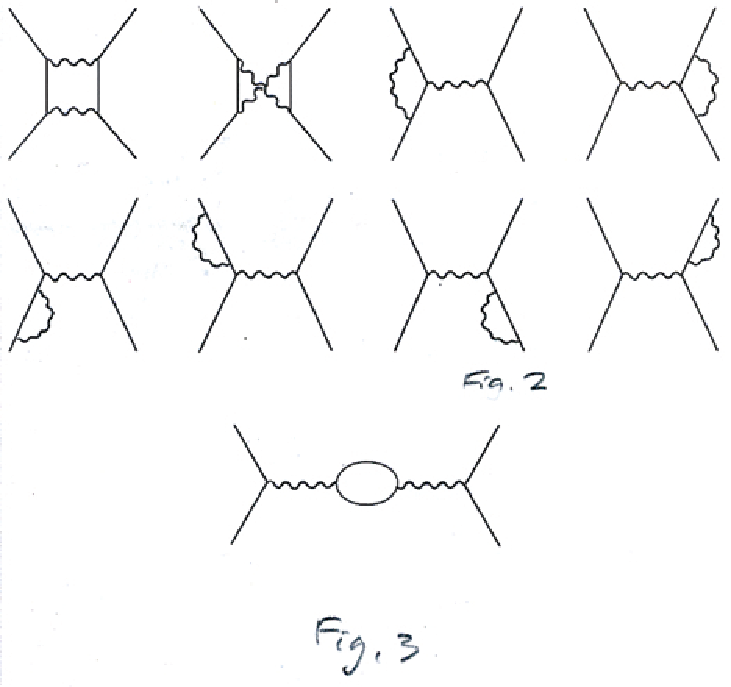
\includegraphics[width=0.98\textwidth]{figs/fig_i1}
\end{center}


Virtual fluctuations of the (electromagnetic) vacuum (see Fig. 4),
\begin{center}
	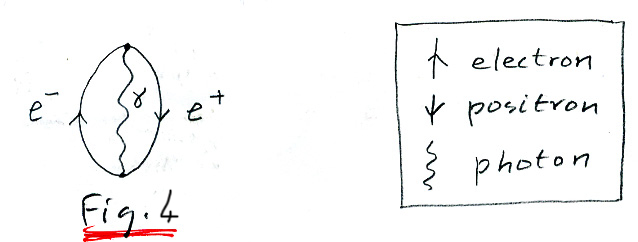
\includegraphics[width=0.6\textwidth]{figs/fig_i2}
\end{center}
corresponding to the ZPF of a harmonic oscillator which contribute for each degree of freedom an energy of $\frac{1}{2}\hbar \omega$ (photon frequency) and which allegedly can lead to a number of effects (viscosity of the vacuum, overshadowing of any matter in the vicinity of a neutron star formation, force an energy like cosmological constant in Einstein's equations, account for a sizable fraction of the hypothized dark matter mechanism in the recession of galaxies, etc) can become real in e.g. the (Lamb) shift of energy levels of the hydrogen atom (Feynman, R.P. (1961) \emph{Quantum Electrodynamics}, Frontiers in Physics, Benjamin, Reading, Mass., Thirtieth Lecture, p. 153--157; Greiner, W. (1998) \emph{Quantum Mechanics}, Special Chapters, Springer Verlag, Heidelberg, p. 149--160) (see Fig. 5).
\begin{center}
	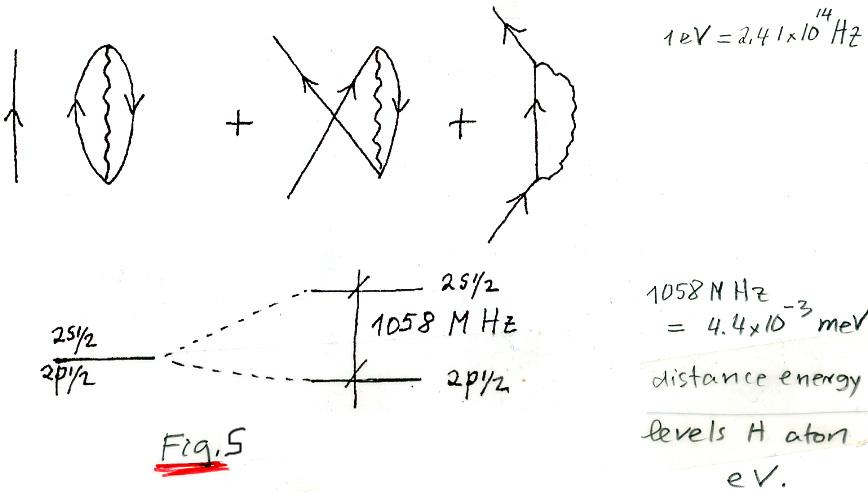
\includegraphics[width=0.98\textwidth]{figs/fig_i3}
\end{center}

Summing up, all of NFT is contained in the (quantal) ground state of the nucleus and associated ZPF (see Fig. 6), in the similar way in which all of QED is contained in the electromagnetic vacuum, and all of evolution of the Universe is contained in the Big Bang.
\begin{center}
	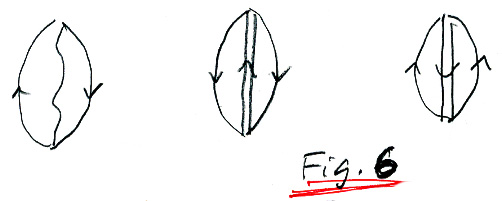
\includegraphics[width=0.6\textwidth]{figs/fig_i4}
\end{center}

Interweaving is at the origin (ZPF). It is not something that comes after. In this sense, ``nothing is bare'' acquires its real sense, and can be directly probed by inelastic, one--particle and two--particle transfer processes (see Figs. 7, 8 and 9, and App. B), all observables are renormalized, and only theoretically can one talk about bare and medium polarization effects separately\footnote{Only, in the very short span in which mean field with collective vibrations is formed.}, as if $\alpha = 1/137$ could be set equal to zero, or $\beta_\lambda (\alpha=0,\pm 2)$.
\begin{center}
	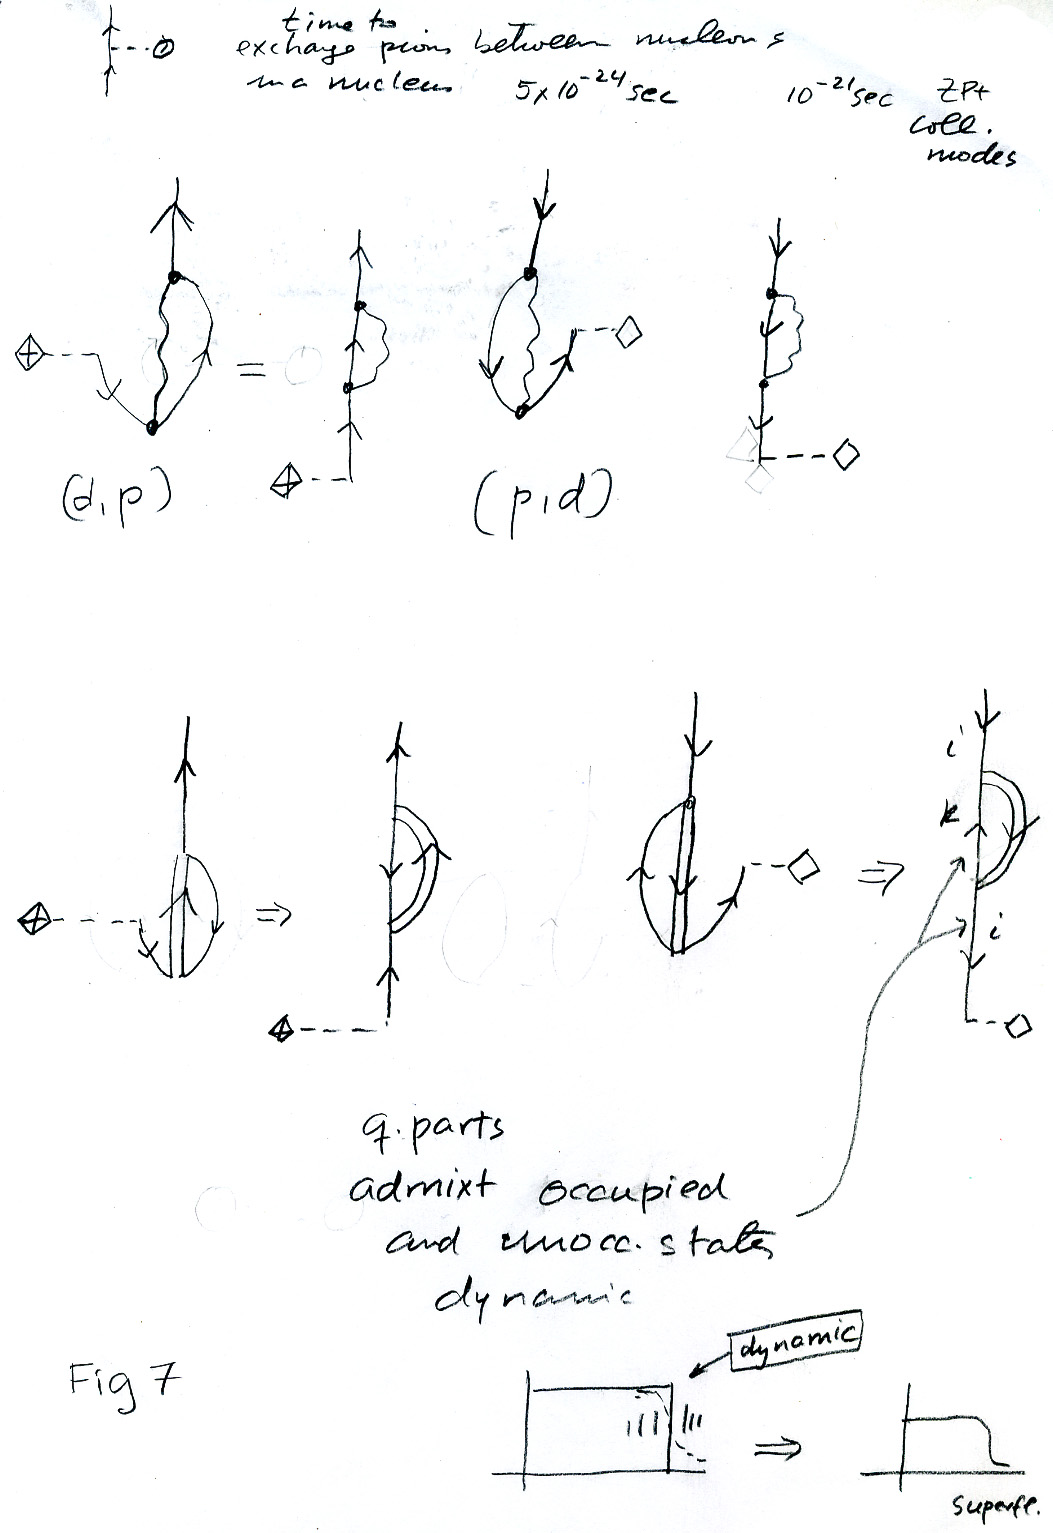
\includegraphics[width=0.88\textwidth]{figs/fig_i5}
\end{center}
\begin{center}
	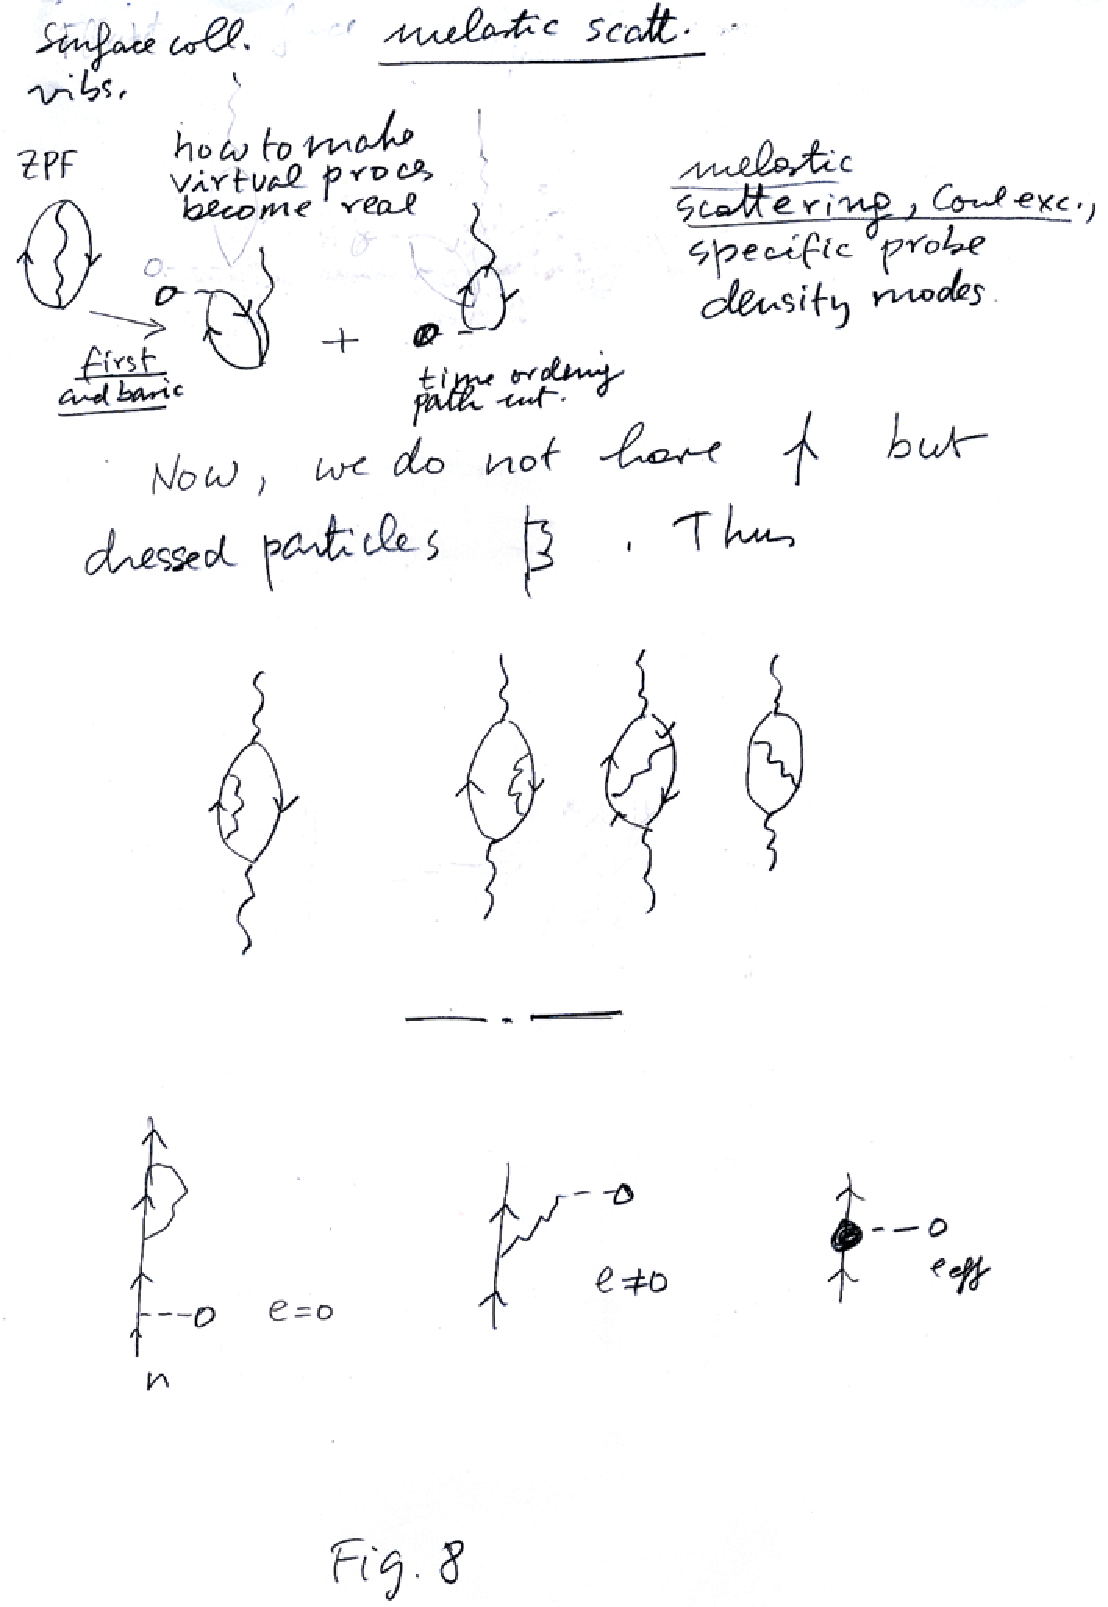
\includegraphics[width=0.98\textwidth]{figs/fig_i6}
\end{center}
\begin{center}
	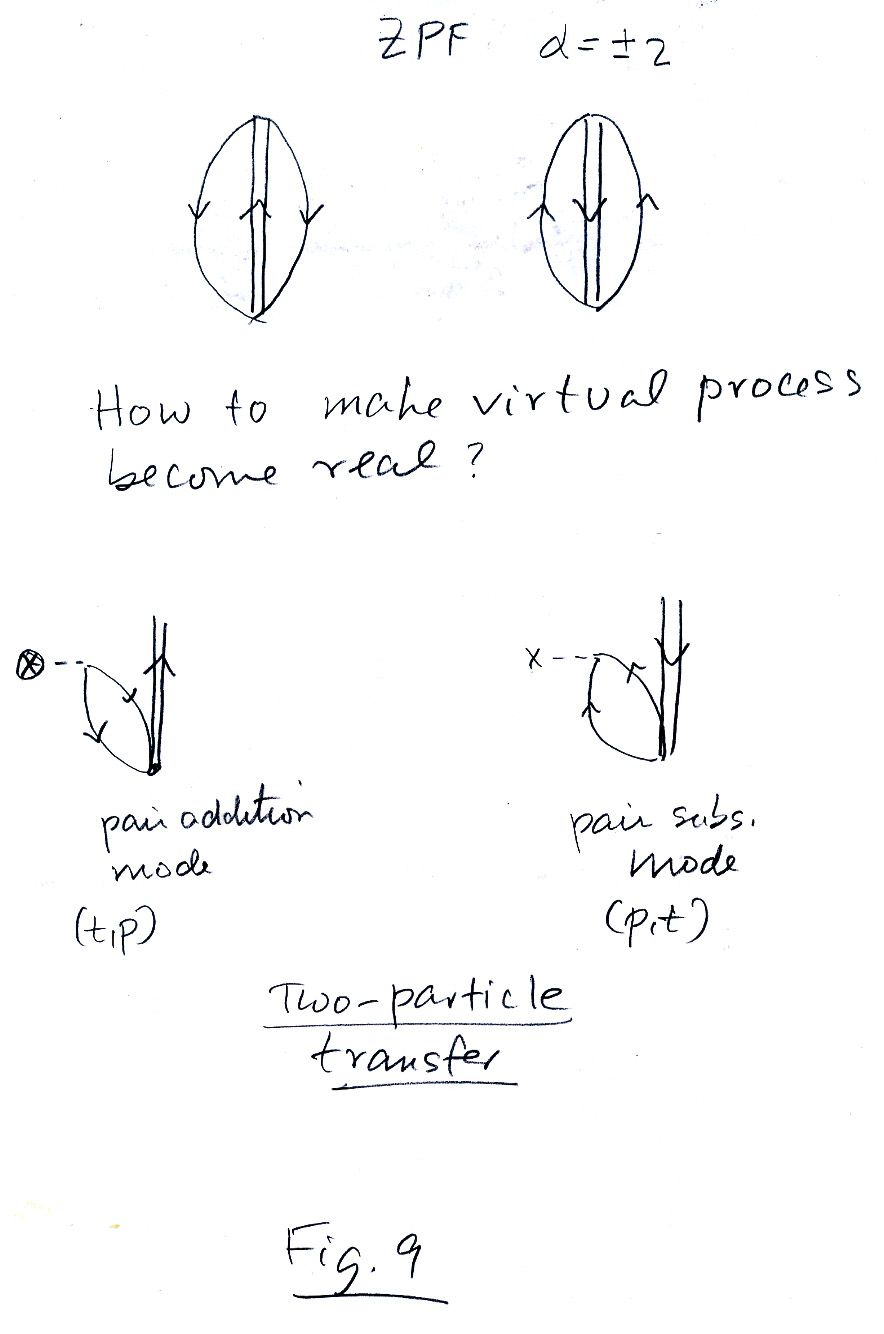
\includegraphics[width=0.98\textwidth]{figs/fig_i7}
\end{center}


\appendix

\pagebreak

%APP A
\section{Spontaneous symmetry breaking, symmetry restoration and ZPF}

The central issue of research is the microscopic interpretation of the spontaneous symmetry breaking phenomenon and associated emergent properties (with models, experiments, eventually some mathematics, but remember that it cannot be exact. And if it is, it is wrong) in different systems (superconductivity in metals, superfluidity in nuclei, spins in paramagnetic systems, amino acid sequence in a protein, etc.). 

\begin{center}\fbox{ZPF}$\leftrightarrow$\fbox{spontaneous symmetry breaking}\end{center}
are not the same, but one is required by the other.

\begin{center}
	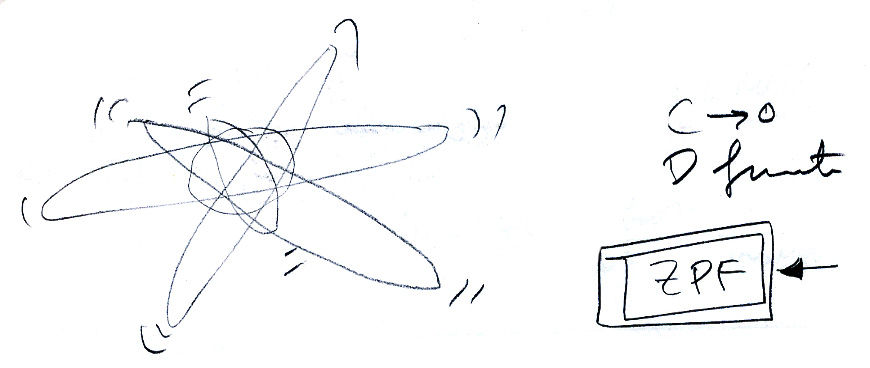
\includegraphics[width=0.98\textwidth]{figs/fig_zpf}
\end{center}

It could not be spontaneous symmetry breaking without fluctuations, as there would not be a mechanism for symmetry restoration, \emph{and a limiting case of ZPF leads to spontaneous symmetry breaking}.

For the discussion of these subjects in terms of a simple model (single $j$--shell description of particle number conservation violation associated with superfluidity in nuclei, see Brink and Broglia 2005, Apps. H and I.


\subsection{Relation between collectivity and correlations}

Let us assume that the collective modes are described in the harmonic approximation. Thus collectivity is measured in terms of the zero point fluctuations (ZPF) of the equivalent harmonic oscillator (see Fig. 1).
\begin{center}
	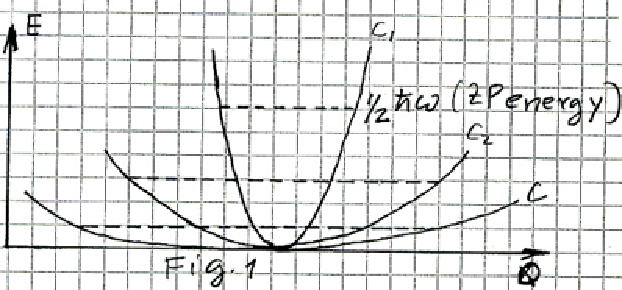
\includegraphics[width=0.98\textwidth]{figs/fig_zpf1}
\end{center}

ZPF (dimensionless parameter)
\begin{equation}
	\langle 0|Q^2|0 \rangle^{1/2} = \sqrt{\frac{\hbar \omega}{2C}} = \sqrt{\frac{\hbar^2}{2D}\frac{1}{\hbar\omega}}
\end{equation}
We assume $C \rightarrow 0$ while $D$ is always finite. The energy of the mode is
\begin{equation}
	\hbar \omega = \hbar \sqrt{\frac{C}{D}}
\end{equation}
while the collectivity is related to
\begin{equation}
	B (0 \rightarrow 1) = \langle 1|Q|0 \rangle^2 = \frac{\hbar \omega}{2C} = \left( \frac{\hbar^2}{2D} \right) \times \left( \frac{1}{\hbar \omega} \right)
	\label{eqn:b01}
\end{equation}
As $C$ decreases collectivity increases. In fact $\hbar \omega \rightarrow 0$ and the transition probability diverges. This in keeping with the fact that the above description also contains the static deformed limit ($C=0$), provided fluctuations are properly treated.

In other words, rotations can be viewed as a vibration with very small restoring constant. In fact, in equation \ref{eqn:b01} the first factor corresponds to the moment of inertia of the rotation while the second is associated with the divergence in the orientation associated with the privileged direction in space defined by the (almost) static deformation (see Fig. 1). In other words, collective is always connected with a dynamic, and in the limit, static, spontaneous symmetry breaking (in the case of Fig. 2 of rotational invariance) and of its restoration.
\begin{center}
	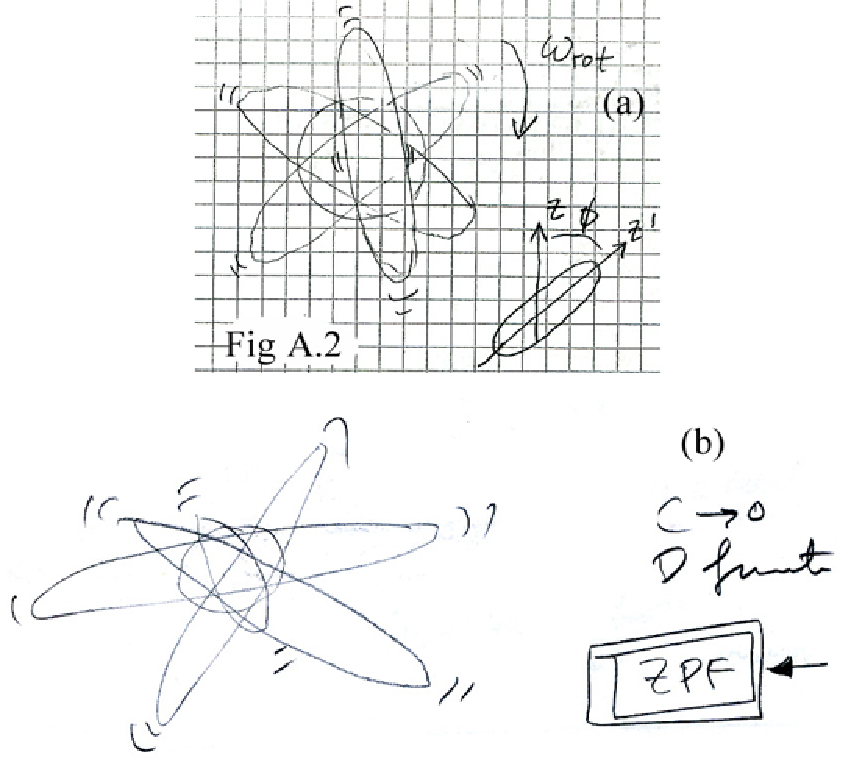
\includegraphics[width=0.58\textwidth]{figs/fig_rotinv}
\end{center}
Divergence of the fluctuations in orientation means that the angle $\phi$ between the laboratory system ($z$) and the body--fixed frame of reference ($z^\prime$) is to be averaged out over the interval $0$--$2\pi$.

Within the harmonic approximation, the microscopic description of collective modes can be made in terms of the RPA, the associate phononic excitation being
\begin{equation}
	|1 \rangle - \Gamma_\alpha^+ = \sum_{ki} \left( X_{ki}^\alpha \Gamma_{ki}^+ + Y_{ki}^\alpha \Gamma_{ki} \right) |0 \rangle \;,
\end{equation}
with
\begin{equation}
	\Gamma_{ki}^+ = a_k^+ a_i
\end{equation}
and
\begin{equation}
	\left. \begin{array}{l} X_{ki}^\alpha \\ Y_{ki}^\alpha \end{array} \right\} = \pm \Lambda \frac{\langle i|F|k \rangle}{(\varepsilon_k - \varepsilon_i) \mp \hbar \omega_\alpha}
\end{equation}
For $C \rightarrow 0$ ($\omega \rightarrow 0$)
\begin{equation}
	|X_{ki}^\alpha| \approx |Y_{ki}^\alpha| \approx \Lambda_\alpha \frac{\langle i|F|k \rangle}{(\varepsilon_k - \varepsilon_i)}
\end{equation}
where the particle--vibration coupling strength is defined as
\begin{equation}
	\Lambda_\alpha = k \sqrt{\frac{\hbar\omega_\alpha}{2C_\alpha}}
\end{equation}
In other words, forwards--going and backwards--going amplitudes become equal, and the ZPF of the system gives rise to an important contribution to the nuclear correlation energy (see Ring and Schuck p. 308--309)
\begin{center}
	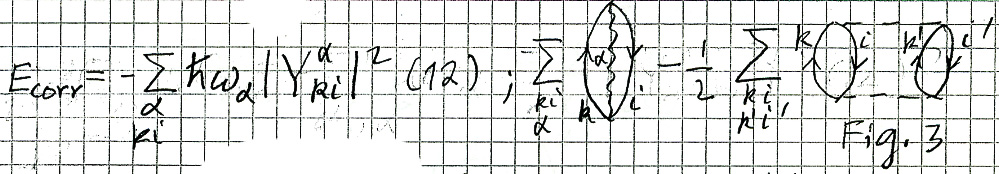
\includegraphics[width=0.98\textwidth]{figs/fig_a3}
\end{center}
From Eqs. (6), (9), (10) and (12) it is seen that there is a close connection between collectivity (Eq. (6)) and correlation (Eq. (12)). The relation between Eq. (1) and the graphs displayed in Fig. 3 is worked out in the appendix.

Of notice that
$$ E_\textrm{corr} \sim -EWSR$$
where
$$ EWSR = \sum_\alpha \hbar \omega_\alpha \left( \frac{\hbar \omega_\alpha}{2C_\alpha}\right) $$

\subsection{Induced interaction}

The exchange of vibrational modes between nucleons moving in time reversal states close to the Fermi energy can be rewritten as (diagonal term)
\begin{center}
	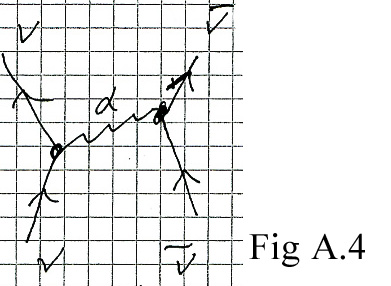
\includegraphics[width=0.78\textwidth]{figs/fig_diagterm}
\end{center}

which again displays similar structure as (6).






\pagebreak

%APP B
\section{One--particle transfer}
If we bring together protons and neutrons to within nuclear interaction range (pion exchange, see Fig. B.1)
\begin{center}
	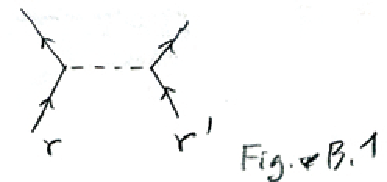
\includegraphics[width=0.48\textwidth]{figs/fig_b1}
\end{center}
it takes $\approx 0.5\times10^{-24}$ sec, for the mean field to be generated, that is (see Fig. B.2)
\begin{center}
	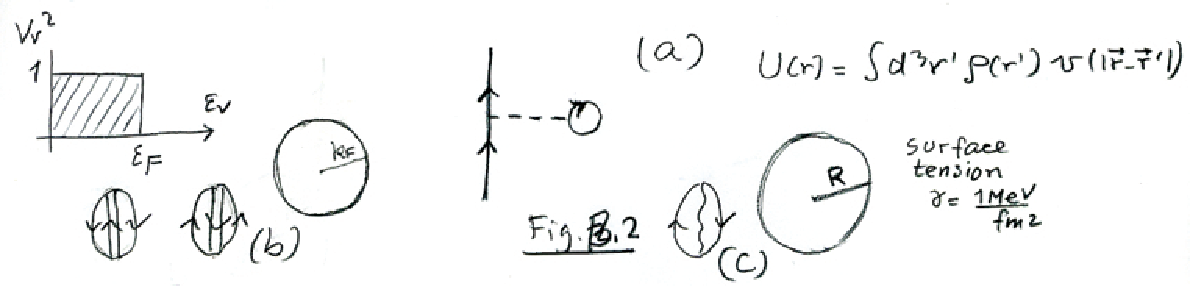
\includegraphics[width=0.98\textwidth]{figs/fig_b2}
\end{center}
and it takes $\approx 0.7\times10^{-21}$ sec for the nuclear surface and the Fermi surface to start displaying ZPF associated with the establishment of $p$--$h$ correlations (surface vibrations with typical energies 1--2 Mev) and of $p$--$p$ or $h$--$h$ correlations (pair addition and pair subtraction modes).

\subsection{Pauli principle}
Let us consider the potential single--particle motion discussed above in presence of ZPF and introduce Pauli corrections in (see Fig. B.3) both the reduction of the two--body interaction (Fig. B.1) into a mean field (Fig. B.2(a)) as well as in connection with the ground state (vacuum), ZPF (Fig. B.2(b) and (c)).
\begin{center}
	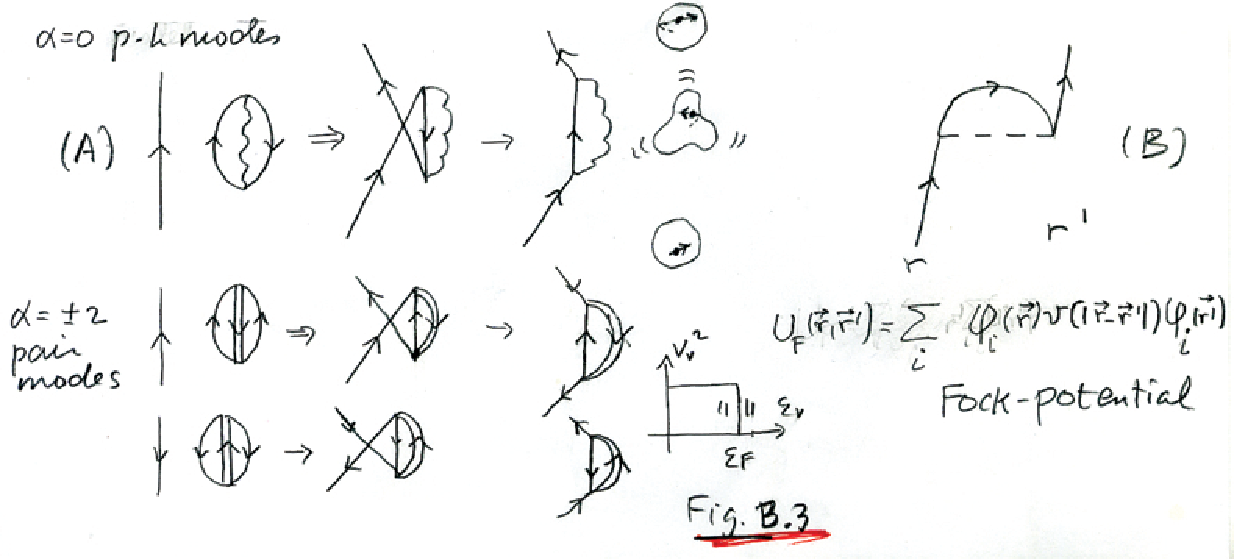
\includegraphics[width=0.98\textwidth]{figs/fig_b3}
\end{center}
The result is the Fock potential (see Fig. B.3(b), as well as dressed particles (Fig. B.3(a)). Let us now make particle pick--up experiments. The process shown in Fig. B.4(a) gives $m_k=m$, as Hartree field only scatters elastically off the surface, nucleons which want to leave the nucleus. That is charges momentum, but not mass. On the other hand, the Fock correction implies that the nucleon changes position, from $\vec{r}\rightarrow\vec{r^\prime}$ instantaneously. This implies that part of the time the nucleon behaves as if it had zero mass. Thus, particle pick--up on such process will lead to $m_k<m$ (see Fig. B.4(b)).
\begin{center}
	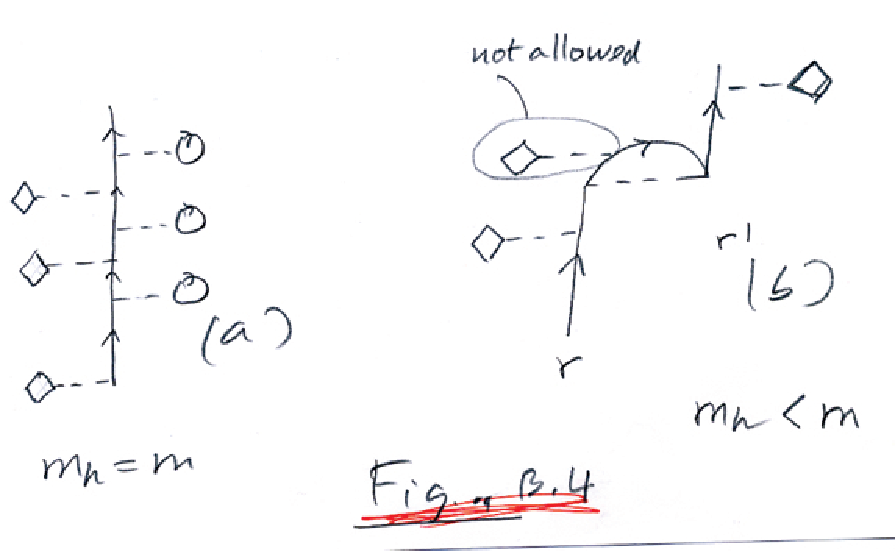
\includegraphics[width=0.98\textwidth]{figs/fig_b4}
\end{center}

Now, pick up of particles dressed by the coupling to surface and pairing vibrations lead to masses $m_\omega > m$, in keeping with the fact that now the nucleon have to carry also the phonons, and their associated inertia (see Fig. B.5), another picture of the same phenomenon is that nucleons move in a gas of surface and of pairing vibrations, which is medium that act with viscosity, changing thus the effective nucleon mass. Now, associated with this dressing process, single--particle states display occupation (spectroscopic) factors $z_\omega$ smaller than 1, in keeping with the fact that $z_\omega = (m/m_\omega)$.
\begin{center}
	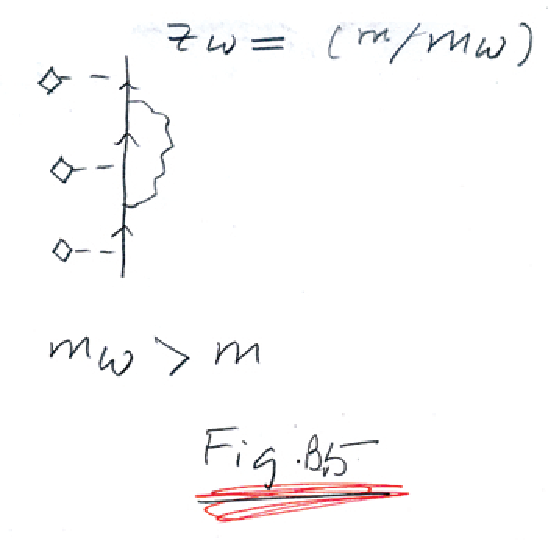
\includegraphics[width=0.68\textwidth]{figs/fig_b5}
\end{center}

The actual values of $m_k$, $m_\omega$ and $m^\star = m_k m_\omega/m$ are discussed in appendix \quad (picket fence model + $k$--mass + $\omega$--mass).



\pagebreak

%APP C
\section{Specific probes: virtual states become real}

In what follows we provide examples of the physics one would like to learn concerning the interweaving of single--particle and collective modes in nuclei, in particular in connection with medium polarization induced pairing interaction. The nucleus ${}^{11}$Li is used as a paradigm of highly polarizable atomic nuclei, and the probes used are one and two--particle pick--up process.
\begin{center}
	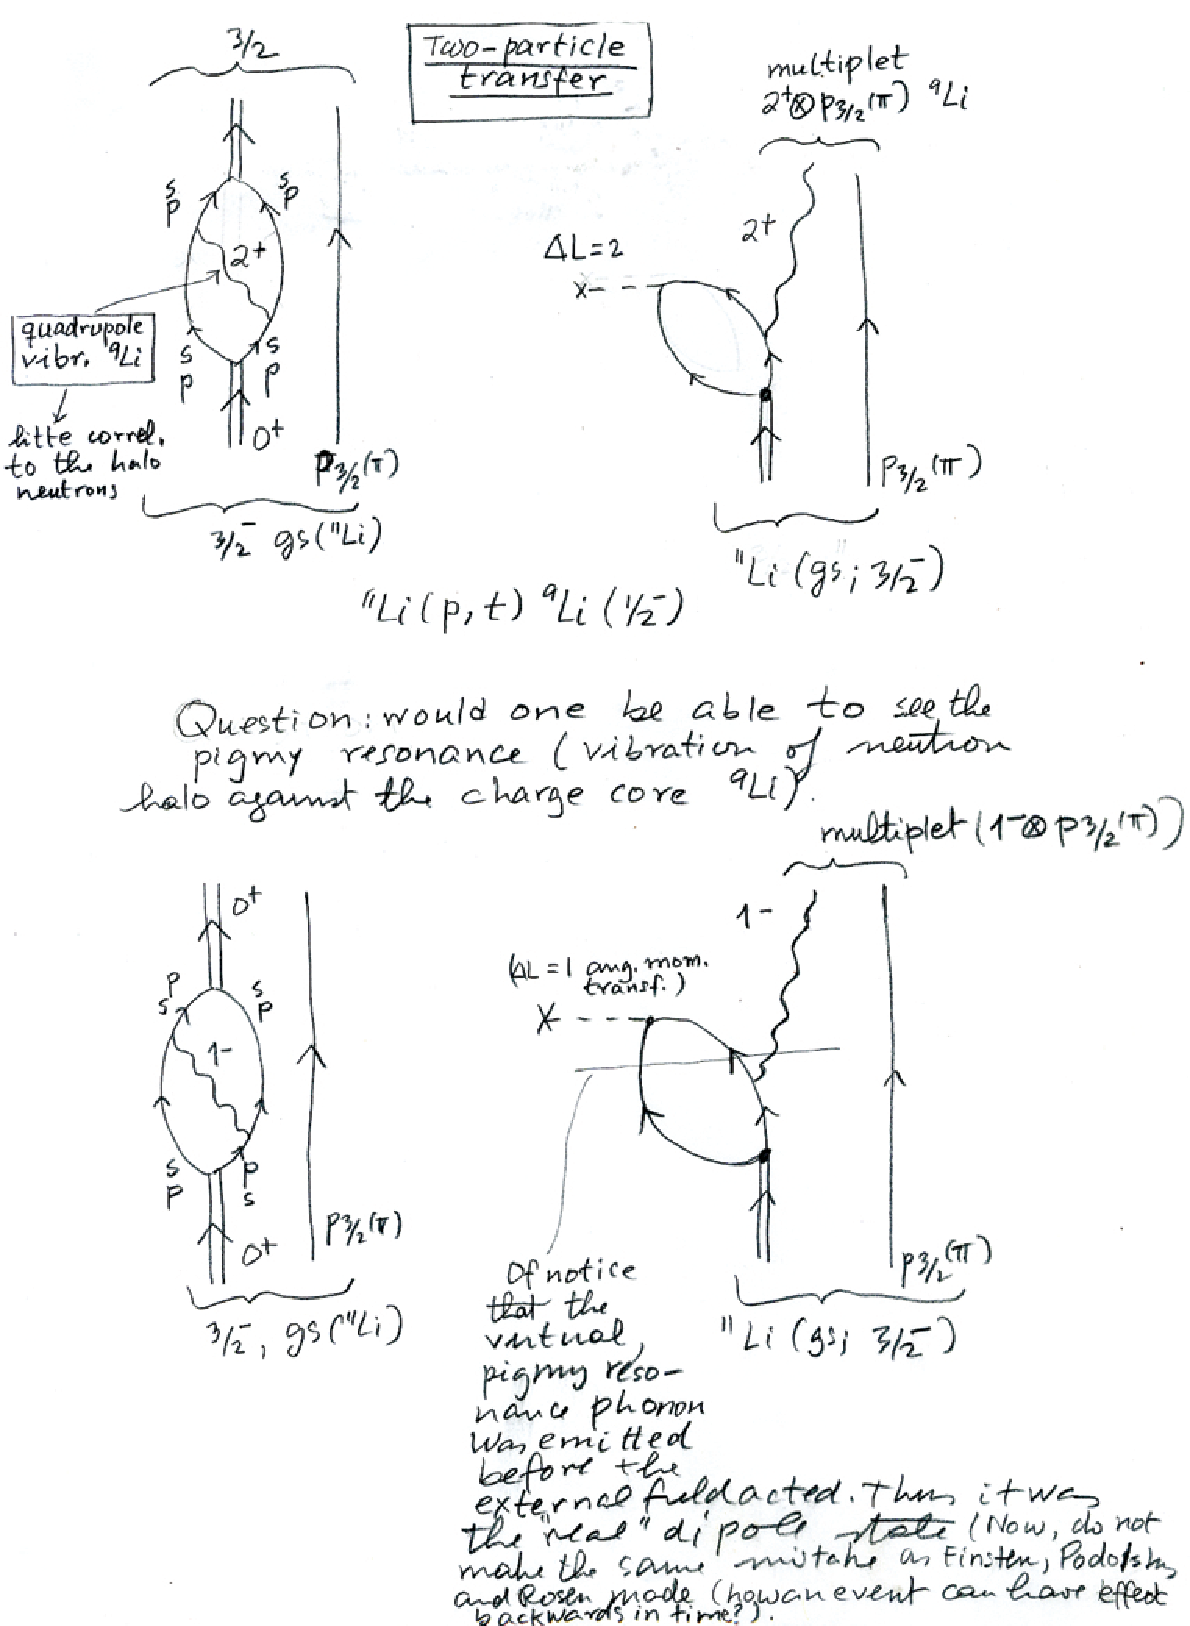
\includegraphics[width=0.98\textwidth]{figs/fig_c1}
\end{center}

\begin{center}
	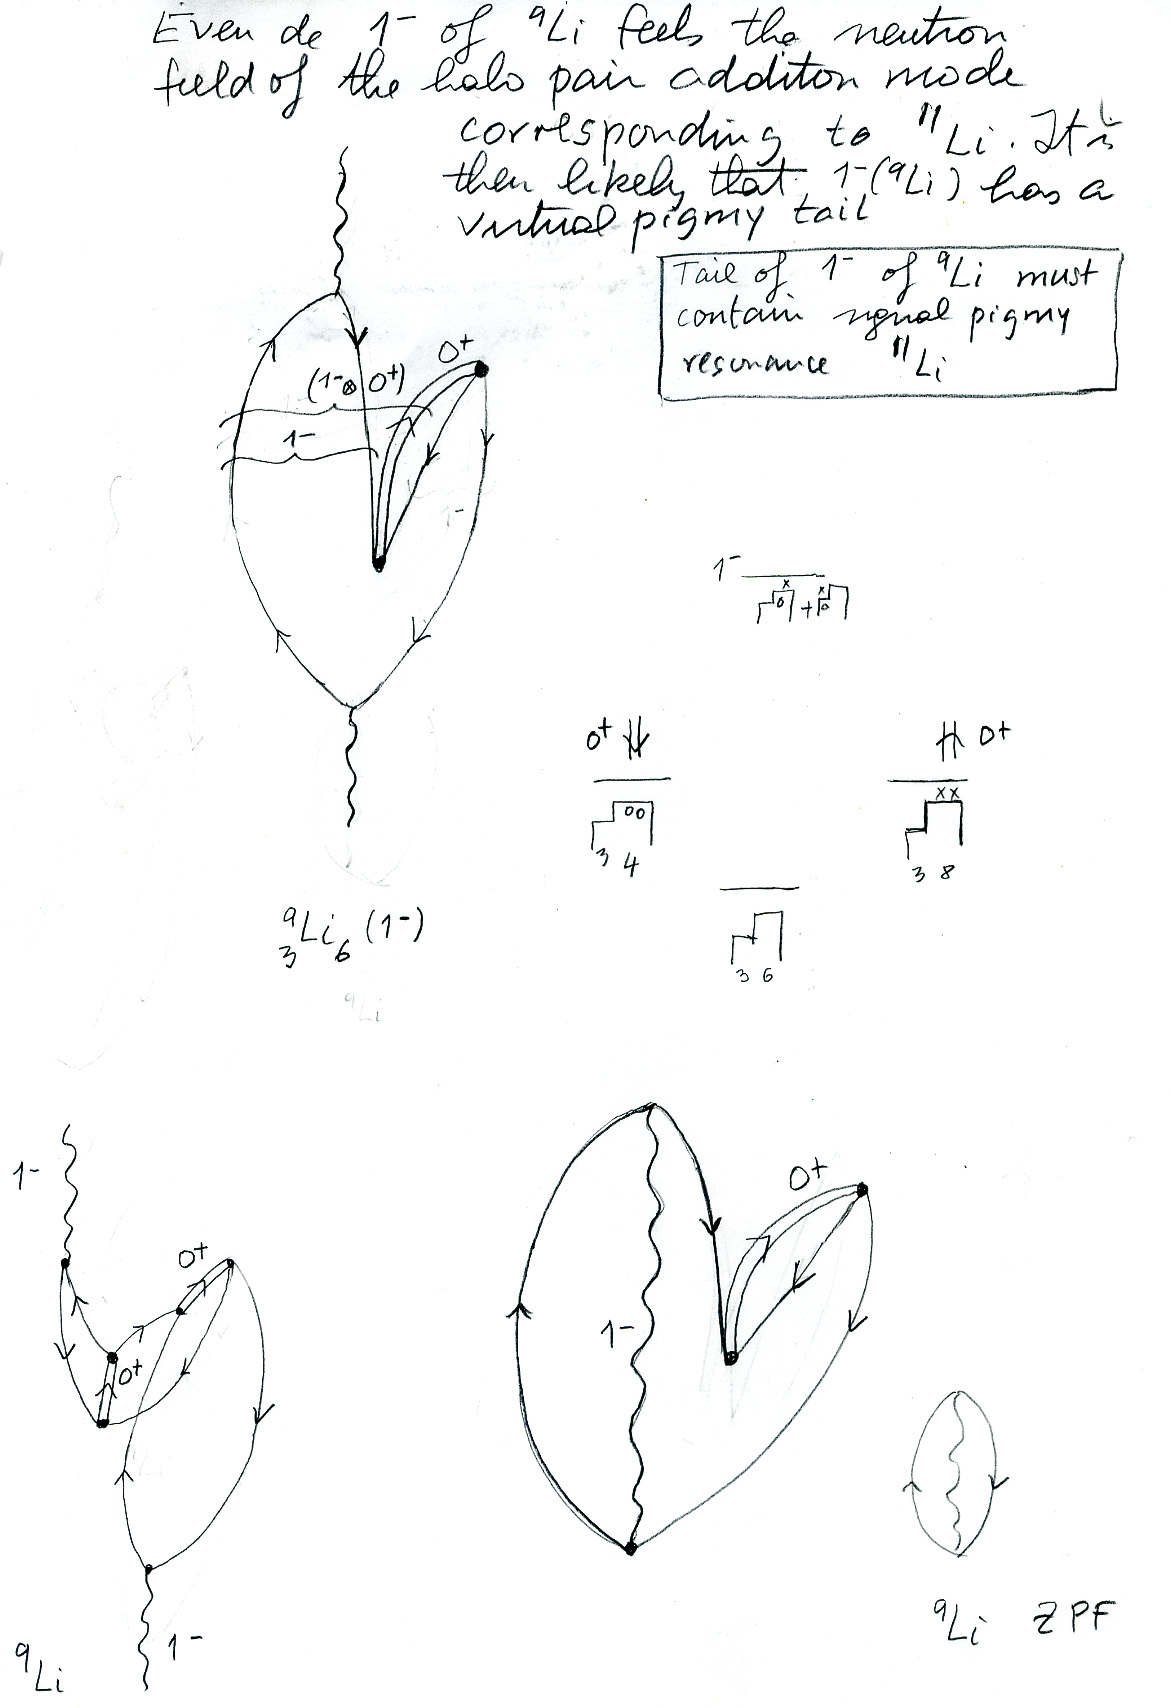
\includegraphics[width=0.98\textwidth]{figs/fig_c2}
\end{center}

\begin{center}
	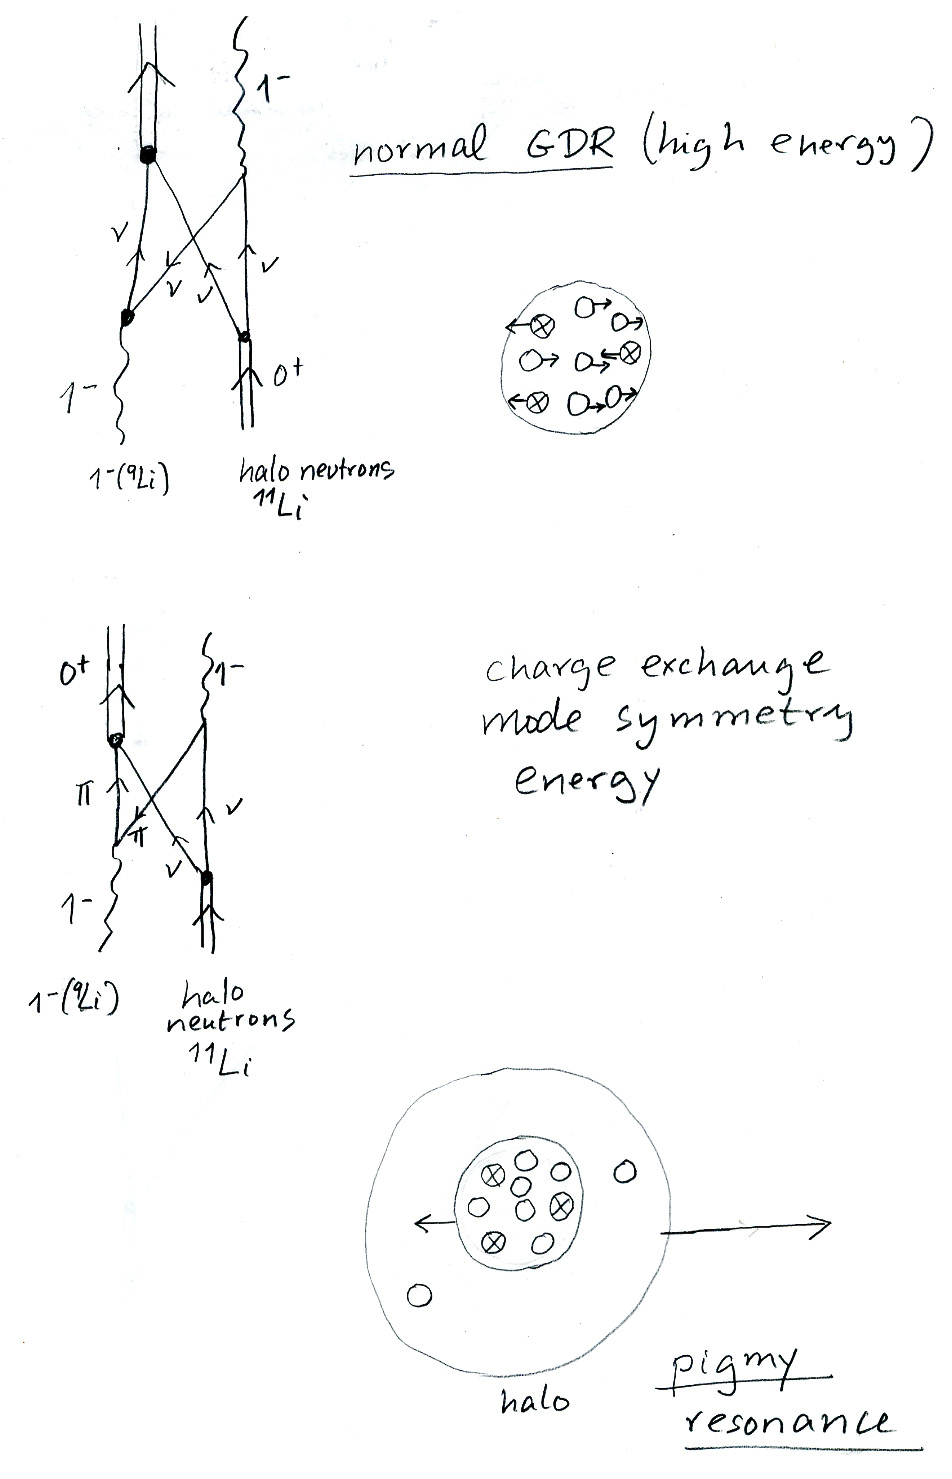
\includegraphics[width=0.98\textwidth]{figs/fig_c3}
\end{center}

\begin{center}
	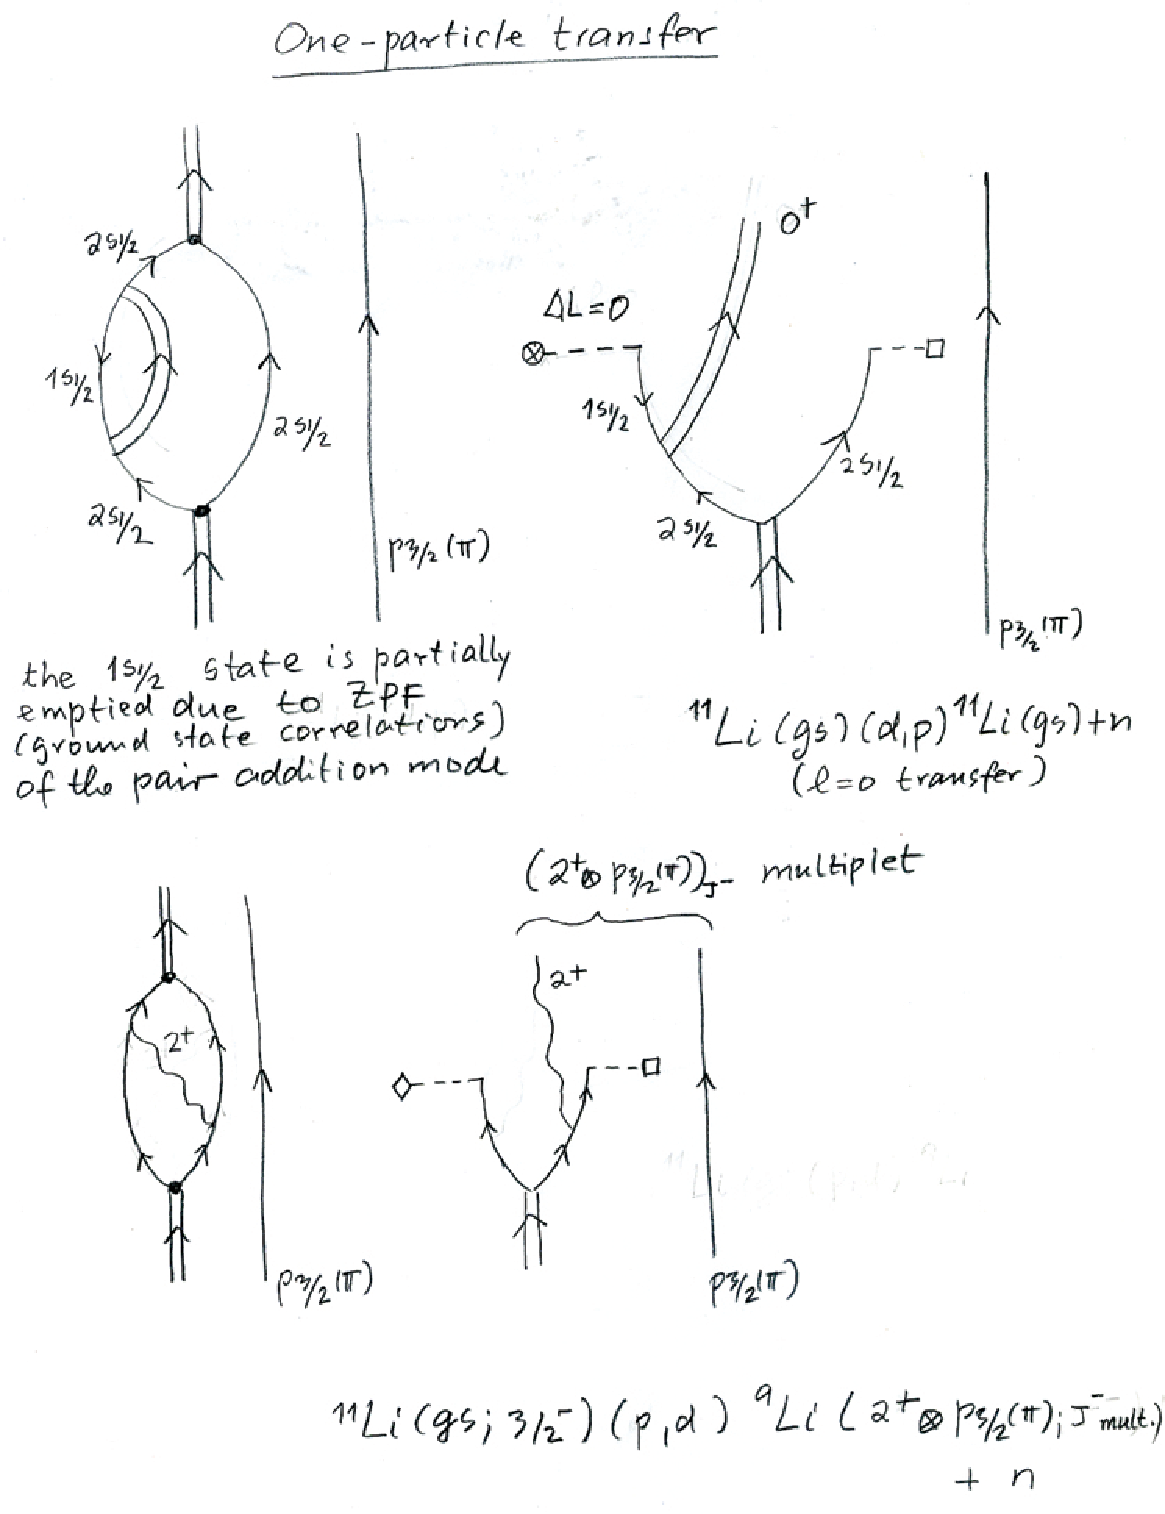
\includegraphics[width=0.98\textwidth]{figs/fig_c4}
\end{center}

\begin{center}
	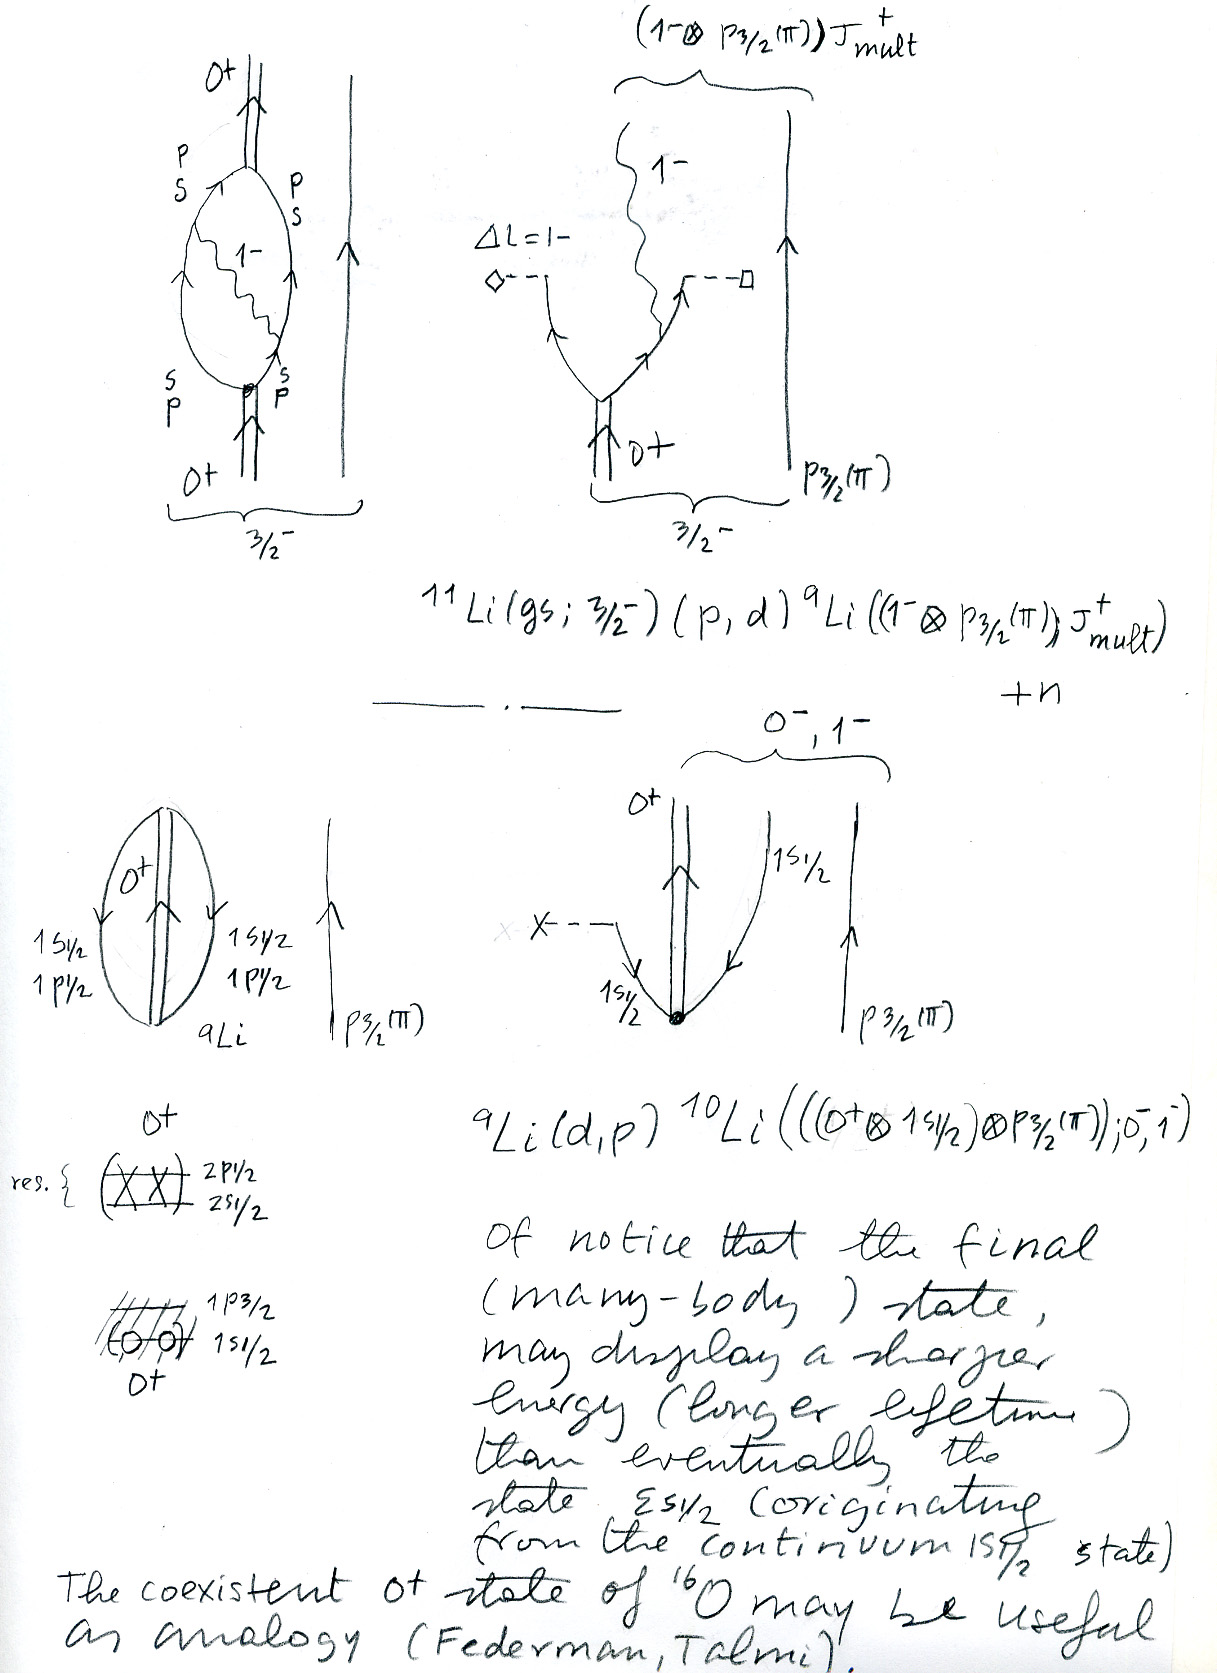
\includegraphics[width=0.98\textwidth]{figs/fig_c5}
\end{center}

\begin{center}
	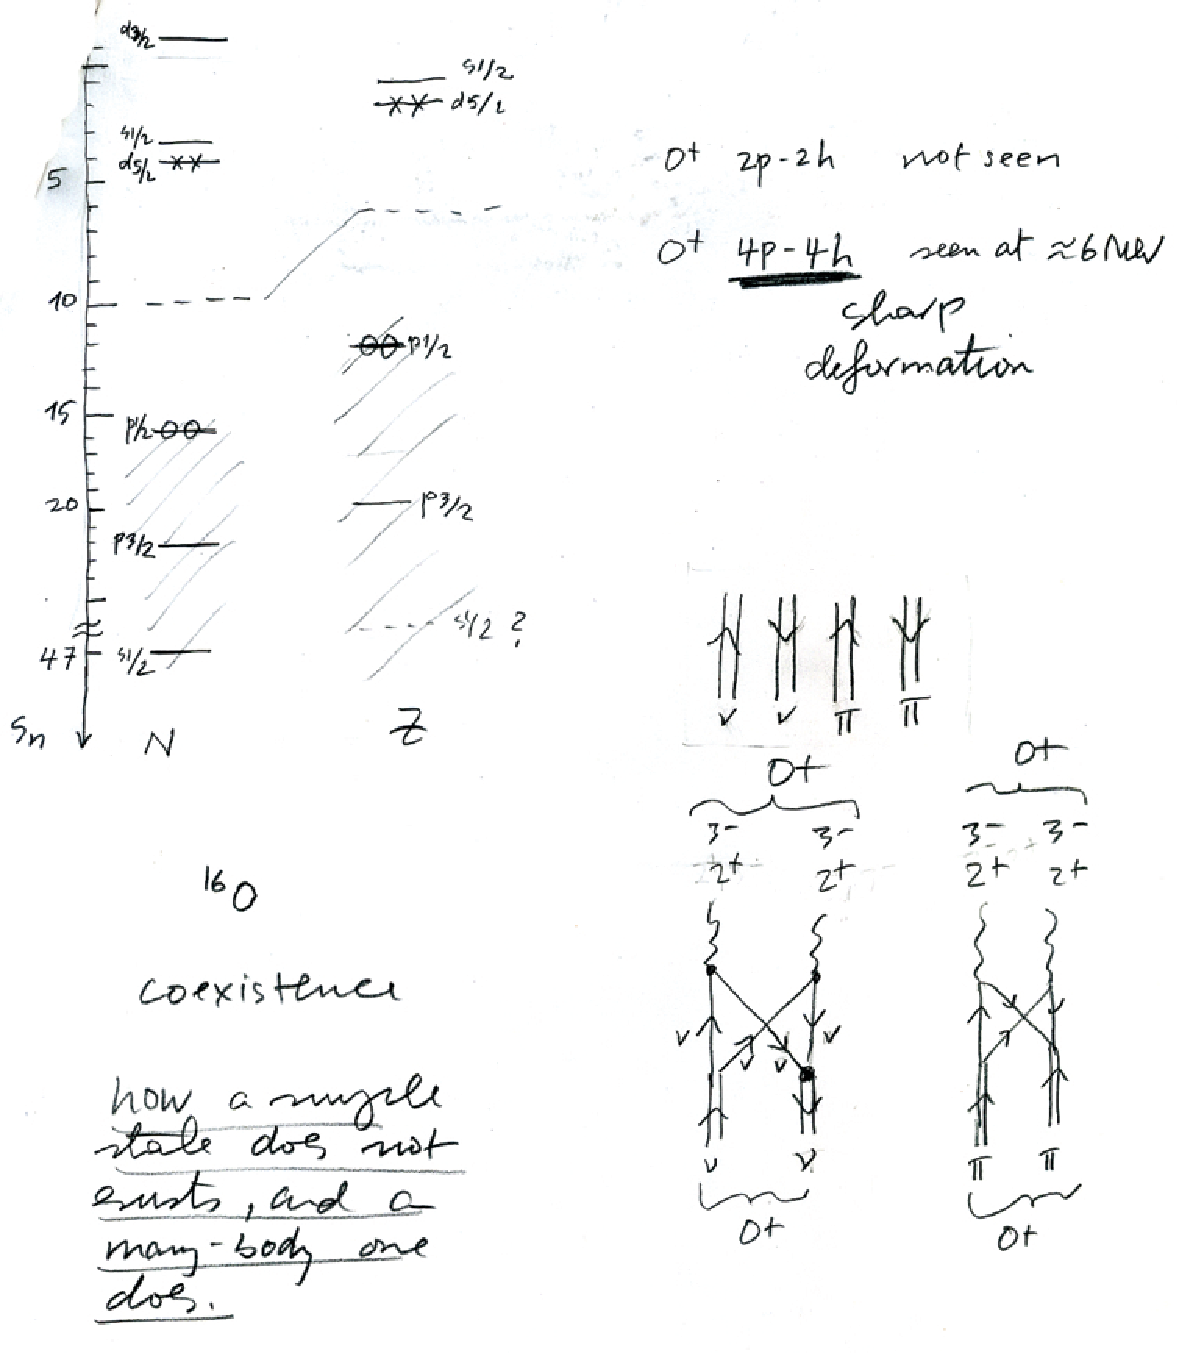
\includegraphics[width=0.98\textwidth]{figs/fig_c6}
\end{center}






\pagebreak

%APP D
\section{Quantality parameter}

\begin{center}
	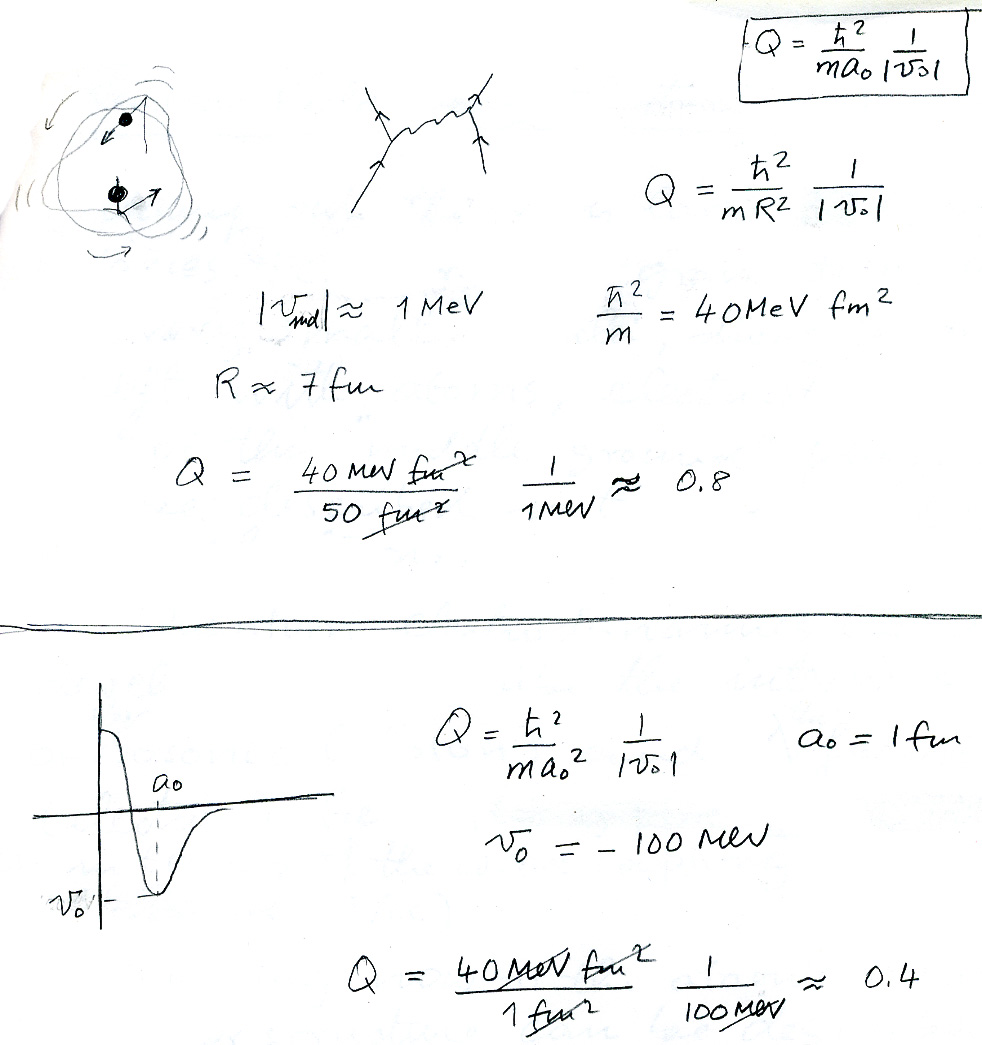
\includegraphics[width=0.98\textwidth]{figs/fig_appd}
\end{center}

From the above estimates, one can conclude that strongly, polarizable nuclei are better independent particle model than close shell nuclei.




\pagebreak

%APP E
\section{The nuclear many--body problem of structure and reactions in a nutshell}

Mean field theory provides the tools to determine a single--particle potential in which nucleons move independently of each other, filling the pullings and pushings of all other nucleons when trying to leave the system, being elastically reflected by the nuclear surface located at a radius $R$ ($\approx 1.2 A^{1/3}$ fm). Associated with this system is a Fermi sphere in which the Fermi momentum $k_F$ is related to the energy difference between the last occupied and the first unoccupied orbitals\footnote{In the case of atomic physics this is known as the Highest Occupied Molecular Orbital (HOMO), the first completely empty state being known as the Lowest Unoccupied Molecular Orbital (LUMO).}. Being the nuclear surface a two--dimensional quantal system, displaying a surface tension of $\approx 1$ MeV/fm, it can vibrate collectively, as testified by the multiphonon, particle--hole like modes, of different multipolarity, which can be excited in inelastic processes.

Similarly, the Fermi energy can fluctuate, giving use to pair addition and pair subtraction modes which can be excited in two--particle stripping and pick--up reactions. Such experiments have revealed a rich multiphonon spectrum around closed shell nuclei, in particular ${}^{208}$Pb.

The associated ZPF (see Fig. 1) modify the ground (vacuum) state of the system, leading to few MeV contributions to the nuclear mass (Baroni et al \qquad; Bertsch et al \qquad).
\begin{center}
	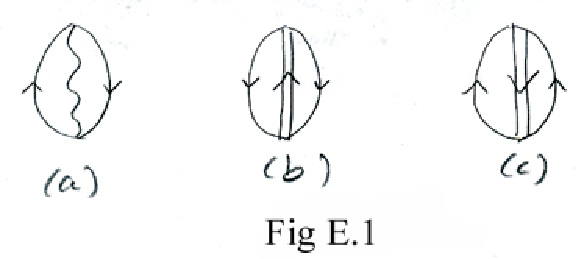
\includegraphics[width=0.58\textwidth]{figs/fig_e1}
\end{center}
To the extent that the vibrations of Fig. 1  can be considered harmonic modes of frequency $\omega_\alpha$, they contribute $1/2 \hbar \omega_\alpha$ for each degree of freedom. Of notice that this energy can be derived from the uncertainty relations existing between $P$ and $Q$, i.e. between the conjugate variables describing the harmonic motion. In other words, quantal ZPF are intimately connected with the uncertainty relations and thus are at the core of quantal phenomena.

Of notice that particles in a potential contribute an energy to the ground state associated with $\Delta x \Delta p_x \geq h$. Consequently, the harmonic (RPA) correlation energy contains both collective and single--particle ZPF. It is then natural that the contribution of the so called oyster diagram (Fig. 1) is equal to $E_\textrm{RPA} - E_\textrm{HF}$.

Now, the different elementary modes of nuclear excitation can be forced from virtual to become real, through inelastic, one--particle and two--particle transfer processes (Fig. 2).
\begin{center}
	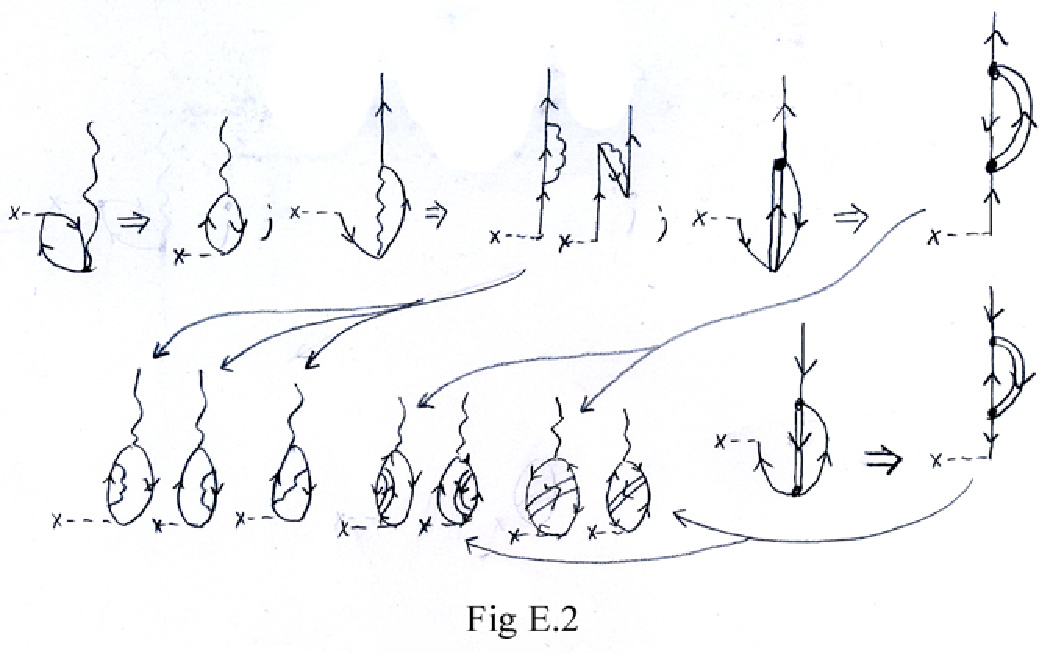
\includegraphics[width=0.98\textwidth]{figs/fig_e2}
\end{center}

Within this framework one has, from the starting, a complete interweaving of all the degrees of freedom. One may calculate more or less accurately the different elementary modes of excitation and their couplings, but in any case one starts with the right physics.

It is of notice that in the case in which ZPF diverge, like e.g in the RPA solution of $H''=H_{sp} + H''_p$ (see Brink and Broglia (2005) App. I), one has pair vibrations with $C \rightarrow 0$ and finite $D$, thus mixing pair addition and pair subtraction modes, and leading to a privileged orientation in gauge space. Because these large amplitude pairing vibrations change orientation in gauge space, with changing frequencies associated with different values of the Fermi energy $\lambda$ (particle number $N$), these fluctuations of orientation of the deformed many--body (superfluid) system in gauge space, restore gauge symmetry, and thus particle number conservation. The goldstone mode associated with spontaneous symmetry violation are pairing rotational bands (see Fig. 3), with energy
$$E_N = AN^2 + \lambda N$$
the associated moment of inertia proportional to $A$ being associated with generalized rigidity.

Summing up, ZPF, indeterminacy relations, and spontaneous symmetry breaking imply each other being, to a large extent, different versions of the same physics.


\subsection{Mean field: spontaneous symmetry breaking}

Let us write the Hamiltonian describing the nuclear system in terms of a separable two--body interaction of constant matrix elements
\begin{align}\label{eqn:e.1}
	H &= H_{sp} + H_\textrm{two--body} \\ \nonumber
	  &= \sum_i \frac{p_i^2}{2 m_i} - G X^+ X 
\end{align}
with 
\begin{equation}
	X^+ = \sum_i x_i \;, 
	\label{eqn:e.2}
\end{equation}
where $x_i$ indicates the coordinate of the $i$--th nucleon. Let us assume that there exists a mean field solution. Let us denote $| MF \rangle$ the corresponding ground state (determinant) wavefunction. It is assumed that
\begin{equation}
	\langle MF|X^+|MF \rangle = \langle MF|X|MF \rangle^* = x_0
	\label{eqn:e.3}
\end{equation}
The above Hamiltonian can then be written as
\begin{align} \label{eqn:e.4}
	-GX^2 &= -G \left[ (X - x_0) + x_0 \right] \left[ (X - x_0) + x_0 \right] \\ \nonumber
		  &= -G \left[ (X - x_0)^2 + 2 x_0 (X - x_0) + x_0^2 \right] \;. 
\end{align}
assume $|GS\rangle$ to be the exact ground wavefunction of $H$. Furthermore, let assume that
\begin{equation}
	\langle GS|(X-x_0)^2|GS\rangle \ll x_0^2 \;.
	\label{eqn:e.5}
\end{equation}
Thus
\begin{equation}
	-GX^2 = -2 \delta X - \frac{\delta^2}{G} + \sigma \left( (X-x_0)^2 \right) ';,
	\label{eqn:e.6}
\end{equation}
where
\begin{equation}
	\delta = G x_0 \;.
	\label{eqn:e.7}
\end{equation}
The mean field, single--particle, interaction can then be written as
\begin{align}\label{eqn:e.8}
	V_{MF} &= -2 \delta X - \frac{\delta^2}{G} \;, \\ \nonumber
		   &= -\delta (X^+ + X) - \frac{\delta^2}{G} \;, 
\end{align}
where $X^+$ is the hermitian conjugate operator to $H$.

In what follows we choose a couple of embodiments of the operator $X$ connected each to important components of the residual nuclear interaction. Let us first assume
\begin{equation}
	X^+ = P^+ = \sum_\nu a_\nu^+ a_{\bar{\nu}}^+ \;.
	\label{eqn:e.9}
\end{equation}

In other words, $X^+$ is now the pair addition mode associated with collective pairing vibrations (fluctuations of particle number in gauge space), while
\begin{equation}
	H_p = H_\textrm{two--body} = -GX^+X = -GP^+P
	\label{eqn:e.10}
\end{equation}
is the pairing interaction.

The relations (\ref{eqn:e.3}), (\ref{eqn:e.7}) and (\ref{eqn:e.8}) become
\begin{equation}
	\langle BCS | P^+ | BCS \rangle = \alpha_0 \;,
	\label{eqn:e.11}
\end{equation}
\begin{equation}
	\Delta = G_{\alpha_0} \;,
	\label{eqn:e.12}
\end{equation}
and
\begin{equation}
	V_p = - \Delta (P^+ + P) - \frac{\Delta^2}{G}
	\label{eqn:e.13}
\end{equation}
constitutes the basis of the so called BCS, mean field, solution of the pairing Hamiltonian (Bardeen, Cooper and Schrieffer (!957a,b)). Equation (\ref{eqn:e.11}) implies that this solution violates gauge invariance (particle number conservation), and that the state $|BCS\rangle$ is a wavepacket in the number of particles, and defines a privileged orientation in gauge space. A realization of this solution is found in the nuclear case in connection, for example, to the ground states of the (superfluid) S${}_n$--isotopes. These states, constitute the members of a pairing rotational band (see e.g. Fig. 4.2, p.88 Brink and Broglia (2005)), associated with fluctuations of orientation in gauge space, and this gauge invariance restoration. They are connected to the $|BCS \rangle$ state through a projection operation, that is,
\begin{equation}
	|N\rangle = | {}^A_{50}\textrm{S}_n \rangle \sim \int \textrm{d}\phi \exp{\frac{i N}{2}\phi} | BCS \rangle_{\mathcal{K}^\prime} \;,
	\label{eqn:e.14}
\end{equation}
where $\phi$ is the gauge angle and $| BCS \rangle_{\mathcal{K}^\prime}$ is the BCS state referred to the intrinsic coordinate system in gauge space. Within this context, an emergent property of the spontaneous symmetry breaking of gauge invariance is generalized rigidity in gauge space. That is, if one pushes on the pole of the (gauge) deformed system, the other pole move instantaneously as in a rigid rotation with moment of inertia $2 \mathcal{I}/\hbar^2 \sim 1/G$. Of course, this property is not found in the original, particle conserving Hamiltonian. In other words, the energy of the members of the pairing rotational band can be written as
\begin{equation}
	E_N = \frac{\hbar^2}{2\mathcal{I}} N^2 + \lambda N \;.
	\label{eqn:e.15}
\end{equation}
Of notice that the term $\lambda N$ (Coriolis force in gauge space) has to be added in the calculation of the total energy, as the single--particle energies are, in the BCS solution, measured with respect to the Fermi energy $\lambda$ ($= \varepsilon_F$).

As a second example we choose
\begin{equation}
	X^+ = Q_{2M}^+ = \sum_{i,k} \langle i || Q_2 || k \rangle \left[ a_k^+ a_i \right]_{2M} \;,
	\label{eqn:e.16}
\end{equation}
where
\begin{equation}
	Q_{2M} = r^2 Y_{2M} ( \hat{r} ) \;.
	\label{eqn:e.17}
\end{equation}
In other words, $X^+$ is now the quadrupole operator, associated with particle--hole collective quadrupole surface vibrations, while
\begin{equation}
	H_{QQ} = H_\textrm{two--body} = - k \left( Q_2^+ Q_2 \right)_{00}
	\label{eqn:e.18}
\end{equation}
is the quadrupole--quadrupole interaction.

The relations
\begin{equation}
	\langle N | Q_{2M} | N \rangle = Q_0 \;,
	\label{eqn:e.19}
\end{equation}
and
\begin{equation}
	V_N = - Q_0 \left( Q^+ + Q \right) + \textrm{const} 
	\label{eqn:e.20}
\end{equation}
constitute the basis of the Nilsson, mean field solutions of the quadrupole--quadrupole Hamiltonian (Nilsson (1955), Nilsson and Ragnarsson (1995)). Eq. (\ref{eqn:e.19}) implies that this solution violates rotational invariance in 3D--space, and that $|N \rangle$ is a wavepacket in angular momentum, defining a privileged orientation in space. Symmetry restoration is associated with fluctuations of this orientation and leads to quadrupole rotational bands. The members of these bands are connected to the Nilsson (intrinsic) state through a projection operation
\begin{equation}
	|IMK \rangle \sim \int \textrm{d}\omega \mathcal{D}_{MK}^I (\omega) |N\rangle_{\mathcal{K}^\prime} \;,
	\label{eqn:e.21}
\end{equation}
where $\omega ( \equiv \phi, \theta, \psi )$ stand for the Euler angles and $|N \rangle_{\mathcal{K}^\prime}$ is the Nilsson state referred to the intrinsic set of references with form an angle $\omega$ with respect to the laboratory system. The energy of the members of the rotational band can be accurately parametrized as
\begin{equation}
	E_I = \frac{\hbar^2}{2 \mathcal{I}} I (I+1) + \omega I \;,
	\label{eqn:e.22}
\end{equation}
the linear term in the angular momentum being added to calculate the total rotational energy, in keeping with the fact that the single--particle Nilsson energies calculated in the intrinsic, rotating frame, were all affected by the Coriolis term $-\omega I$, where $\omega$ is the rotational frequency.

An emergent property of the spontaneous symmetry breaking of rotational invariance in 3D--space associated with the Nilsson solution of the quadrupole Hamiltonian is the moment of inertia $\mathcal{I}$, implying generalized rigidity. That is, the possibility of instantaneously propagating a push given in one of the poles of the (assially symmetric) quadrupole deformed system by an inhomogeneous Coulomb and/or nuclear field to the other pole, when setting the system in rotation. Of notice that the relations (\ref{eqn:e.16}) and (\ref{eqn:e.22}) testify to the fact that ``pairing'' and ``quadrupole'' rotational bands are the goldstone modes associated with spontaneous symmetry breaking in gauge (2D) and normal $(x,y,z)$ (3D) space. On the other hand, the relations (\ref{eqn:e.10}) and (\ref{eqn:e.20}) show that two--particle transfer and inelastic and/or Coulomb excitation processes are the specific probes of the phenomena and emergent properties associated with the two particular cases of spontaneous symmetry breaking.

Summing up, the mean field solutions of the total Hamiltonian, violating the different symmetries respected by it, gives rise to single--particle and collective (symmetry restoring) nuclear motion, and of its (intrinsic) interweaving.

An illustration of the parallel between gauge and rotational invariance symmetry breaking and of its consequences is displayed in Table E.1.

\pagebreak
Table E.1 (1)
\begin{center}
	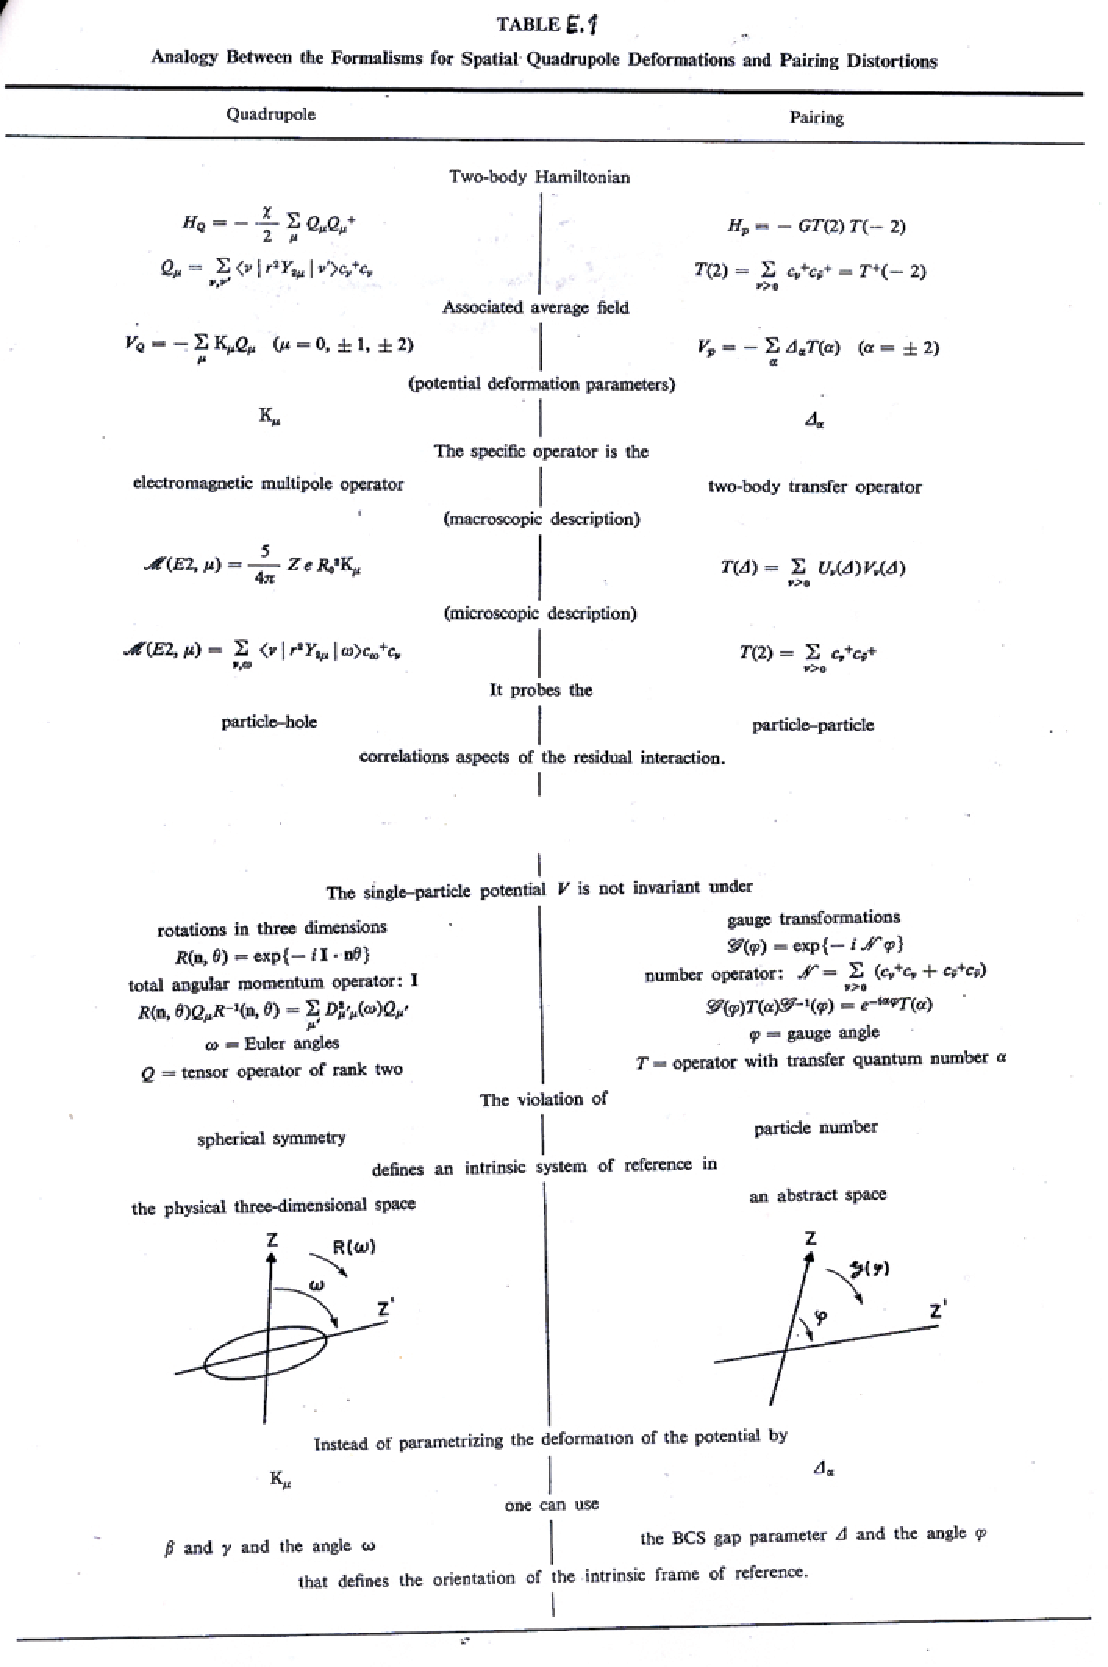
\includegraphics[width=0.98\textwidth]{figs/tab_e1_1}
\end{center}

\pagebreak
Table E.1 (2)
\begin{center}
	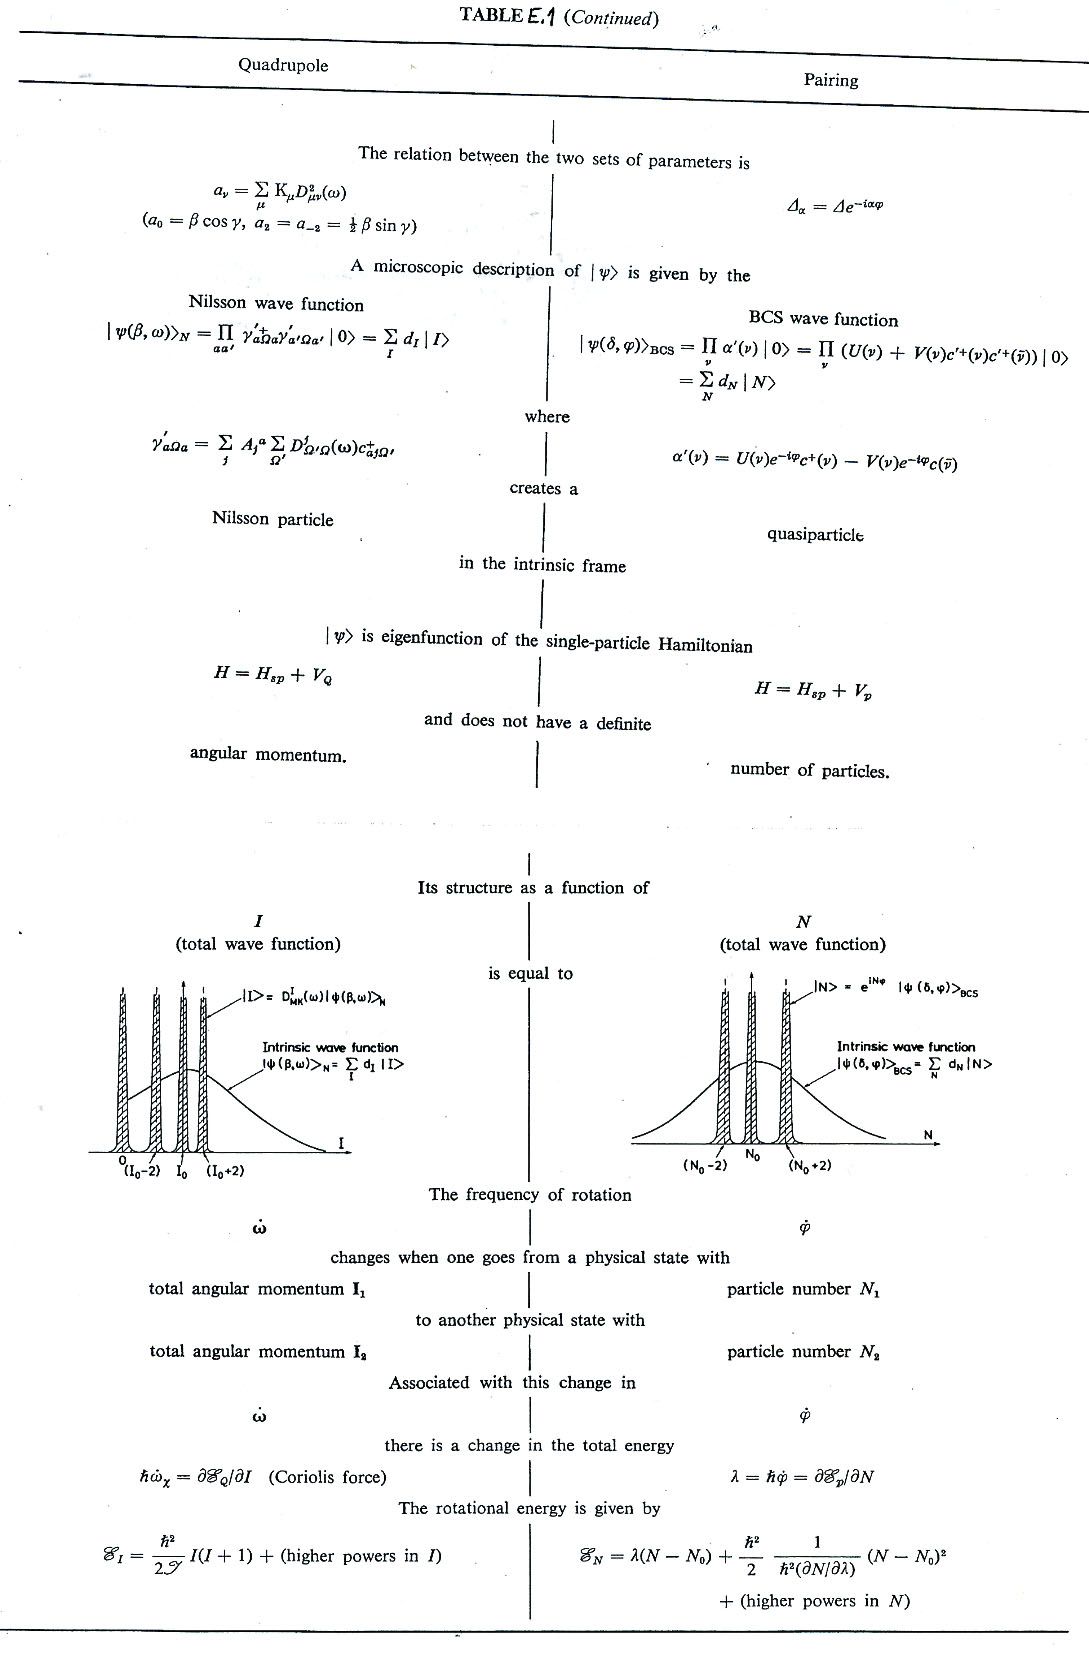
\includegraphics[width=0.98\textwidth]{figs/tab_e1_2}
\end{center}

\pagebreak
Table E.1 (3)
\begin{center}
	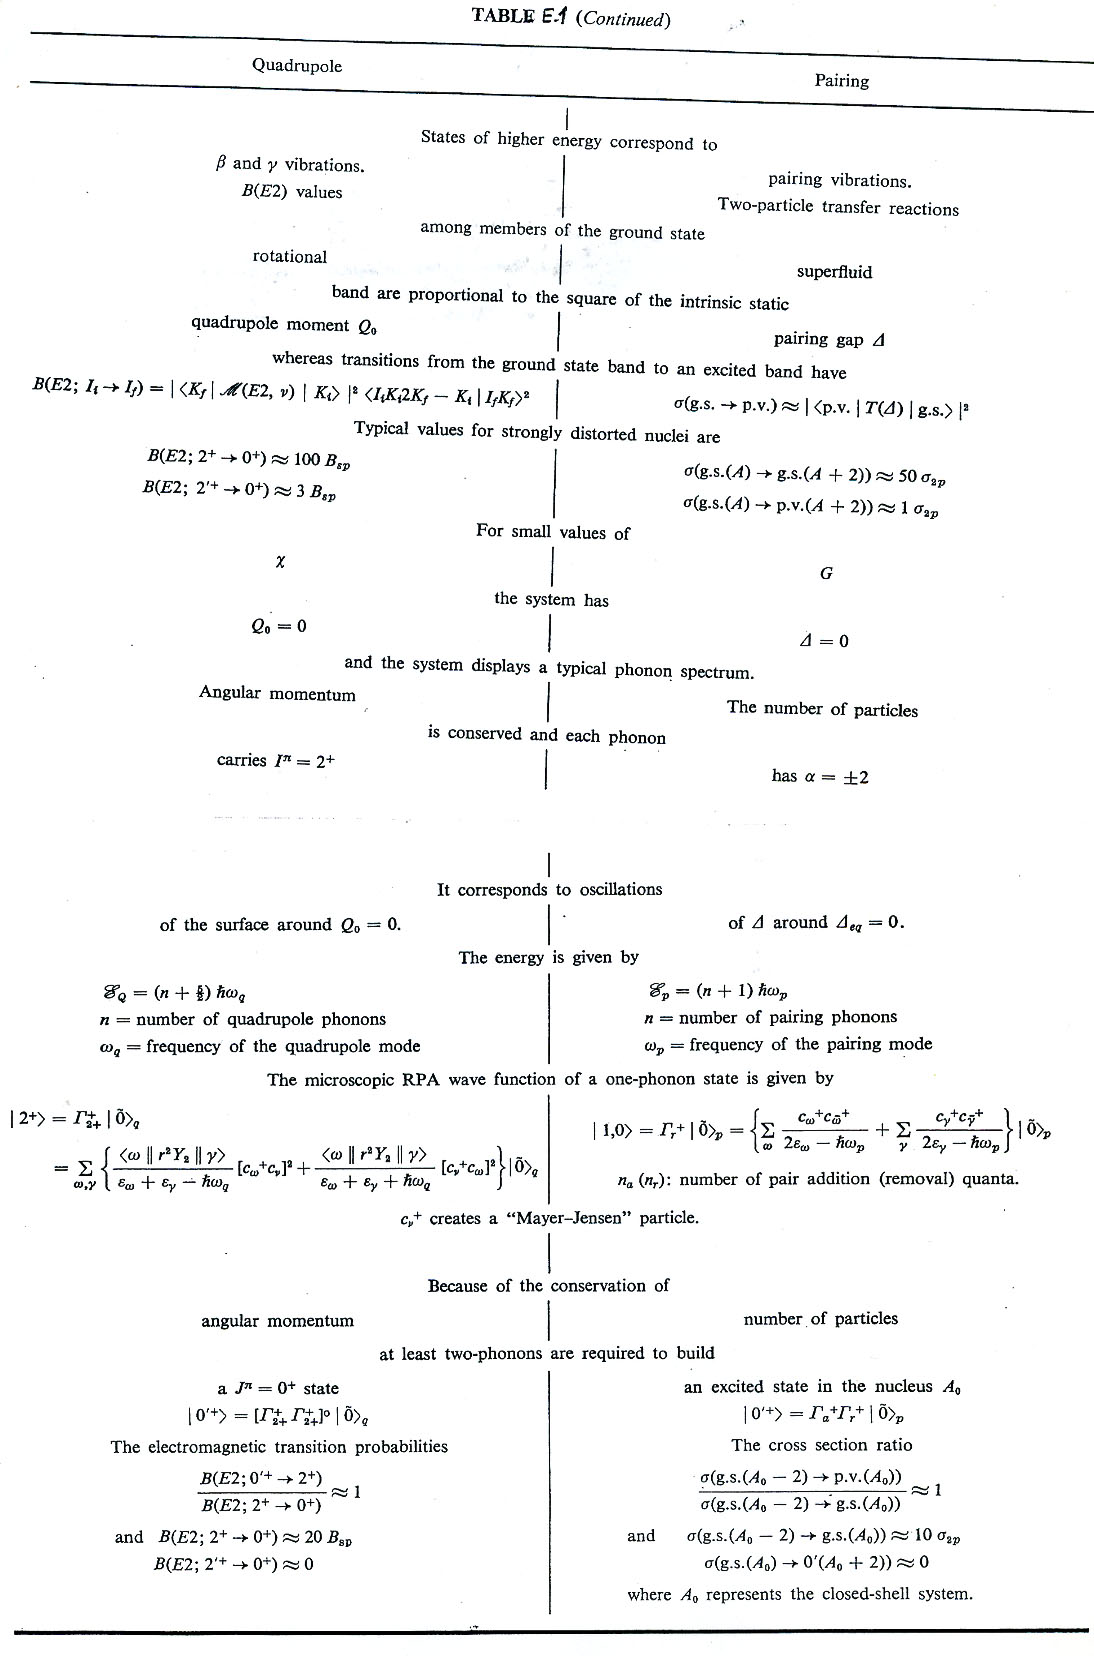
\includegraphics[width=0.98\textwidth]{figs/tab_e1_3}
\end{center}




\pagebreak

\subsection{The pushing model}

\pagebreak

\subsection{The pushing model revisited. Giant dipole resonances, sum rules, effective charges, plasmons, screening.}

Bohr and Mottelson, Vol II (6.15) p. 332.

$(0)$: The superscript $(0)$ refers to the unperturbed $R$ (independent particle--hole excitations)

$$ \alpha_0 = \left( \frac{\hbar \omega}{2C} \right)^{1/2} = \left( \frac{\hbar}{2D \omega} \right)^{1/2} = \left( \frac{\hbar^2}{4CD} \right)^{1/4} $$

$$ \omega = \left( \frac{C}{D} \right)^{1/2} $$

$$ H^{(0)} = \frac{1}{2D^{(0)}} \pi^2 + \frac{C^{(0)}}{2} \alpha^2 $$

$$ C^{(0)} = \frac{\hbar \omega^{(0)}}{2 \left( \alpha_0^{(0)} \right)^2} \qquad D^{(0)} = \frac{\hbar}{2 \omega^{(0)} \left( \alpha_0^{(0)} \right)^2} $$

$$ \sqrt{\frac{C^{(0)}}{D^{(0)}}} = \left( \frac{\hbar \omega^{(0)} 2 \omega^{(0)} \left( \alpha_0^{(0)} \right)^2}{\left( \alpha_0^{(0)} \right)^2 \hbar} \right)^{1/2} = \omega^{(0)} $$

Particle--vibration coupling

$$ H^\prime = \frac{1}{2} K F \alpha = \frac{1}{2} K \alpha^2 $$

\vspace{-0.8cm}

\begin{align*}
	H &= H^{(0)} + H^\prime \qquad \qquad \textrm{(measure with respect to ZPM of unperturbed system)} \\
	&= \frac{1}{2D^{(0)}} \pi^2 + \frac{C^{(0)}}{2} \alpha^2 + \frac{1}{2} K \alpha^2 \\
	&= \frac{\pi^2}{2D^{(0)}} + \left( \frac{C^{(0)}}{2} + \frac{K}{2} \right) \alpha^2 = \frac{\pi^2}{2D^{(0)}} + \frac{\left( C^{(0)} + K \right)}{2} \alpha^2 \\
	&= \frac{\pi^2}{2D} + \frac{C}{2} \alpha^2
\end{align*}

\fbox{
	\begin{minipage}{0.17\textwidth}
		\vspace{-0.6cm}
		\begin{align*}
			D &= D^{(0)} \\
			C &= C^{(0)} + K
		\end{align*}
	\end{minipage}
}

we are thinking about the response of a system to the action of an instantaneous external field.

%\begin{center}
%	\includegraphics[width=0.98\textwidth]{figs/fig_e1_fd}
%\end{center}
\vspace{2cm}

$$ \tilde{F} = e_\textrm{eff} z \;; \quad \begin{array}{l} F = e(EI) z \\ e(EI) = -\frac{e}{2} \tau_z \end{array} $$
$$ \tau_z = \begin{cases} +1\;n \\ -1\;p\end{cases} $$
$$ \alpha = \left( \frac{\hbar \omega_\alpha}{2C_\alpha} \right) \left( \Gamma_\alpha^+ + \Gamma_\alpha \right) = \alpha_0 ( \Gamma^+ + \Gamma )$$
$$ \alpha_0 = \left( \frac{\hbar \omega_\alpha}{2C} \right) $$
$$ \Lambda_\alpha = -K \alpha_0 $$
\begin{align*} 
	&\textrm{(a)} \quad \langle \nu^\prime | \tilde{F} | \nu \rangle = e_\textrm{eff} \langle \nu^\prime | z | \nu \rangle \\
	&\textrm{(b)} \quad \langle \nu^\prime | F | \nu \rangle = e \langle \nu^\prime | z | \nu \rangle \\
	&\textrm{(c)} \quad \frac{\Lambda_\alpha \langle \nu^\prime | F | \nu \rangle \alpha_0}{\varepsilon_{\nu^\prime} - \left( \varepsilon_\nu + \hbar \omega_\alpha \right)} = - \frac{\Lambda_\alpha \langle \nu^\prime | F | \nu \rangle \alpha_0}{\left( \varepsilon_\nu \varepsilon_{\nu^\prime} \right) - \hbar \omega_\alpha} \\
	&\textrm{(d)} \quad \frac{\Lambda_\alpha \langle \nu^\prime | F | \nu \rangle \alpha_0}{\varepsilon_\nu - \left( \varepsilon_{\nu^\prime} + \hbar \omega_\alpha \right)} = - \frac{\Lambda_\alpha \langle \nu^\prime | F | \nu \rangle \alpha_0}{\left( \varepsilon_\nu \varepsilon_{\nu^\prime} \right) - \hbar \omega_\alpha} 
\end{align*}

$$ \langle \nu^\prime | \tilde{F} | \nu \rangle = \langle \nu^\prime | F | \nu \rangle \left( 1+ \chi(F) \right) \qquad F = ez \; \textrm{dipole operator} $$

\begin{align*} 
	\chi(F) &= - \frac{\Lambda_\alpha \langle \nu^\prime | F | \nu \rangle \alpha_0}{\left( \varepsilon_\nu \varepsilon_{\nu^\prime} \right) - \hbar \omega_\alpha} + - \frac{\Lambda_\alpha \langle \nu^\prime | F | \nu \rangle \alpha_0}{\left( \varepsilon_\nu \varepsilon_{\nu^\prime} \right) + \hbar \omega_\alpha} \\
	&= - - \frac{\Lambda_\alpha \langle \nu^\prime | F | \nu \rangle \alpha_0 2 \hbar \omega_\alpha}{\left( \varepsilon_\nu \varepsilon_{\nu^\prime} \right)^2 - \left( \hbar \omega_\alpha \right)^2} = -\frac{K}{C} \frac{\left( \hbar \omega_\alpha \right)^2}{\left( \hbar \omega_\alpha \right)^2 - \left( \varepsilon_\nu \varepsilon_{\nu^\prime} \right)^2}
\end{align*}

$$ \langle \nu^\prime | \tilde{F} | \nu \rangle e_\textrm{eff} \langle \nu^\prime | z | \nu \rangle = e(EI) \langle \nu^\prime | z | \nu \rangle \left( 1 + \chi(F) \right) $$

\begin{center}
	\framebox{
		\begin{minipage}{0.25\textwidth} 
			\vspace{-0.7cm}
			$$ e_\textrm{eff} = - \frac{e}{2} \tau_z \left( 1 + \chi(F) \right) $$
		\end{minipage}
	}
\end{center}

$$ \Delta E = \left( \varepsilon_\nu \varepsilon_{\nu^\prime} \right) \ll \hbar \omega_\alpha  \qquad \textrm{static limit of polarizability} $$

\begin{center}
	\framebox{
		\begin{minipage}{0.3\textwidth} 
			\vspace{-0.5cm}
			$$ \chi(F) = - \frac{K}{C} = - \frac{K}{C^{(0)} + K} $$
		\end{minipage}
	}
\end{center}

\vspace{2cm}

p.387 B+M Vol II Eq (6--123).

The electric multipole moment can be written as a combination of isoscalar and isovector moments.

\begin{align*}
	\mathcal{M}(E\lambda, \mu) &= \int P_\textrm{el} \left( \vec{r} \right) r^\lambda Y_{\lambda \mu} \textrm{d}^3 r \\
	&= \frac{e}{2} \left( \mathcal{M}(\tau=0, \lambda\mu) - \mathcal{M}(\tau=1, \lambda\mu) \right)
\end{align*}

$$ eZ = e \begin{array}{c} \tau=0 \\ \frac{(N+Z)}{2} \\ \textrm{\scriptsize center of} \\ \textrm{\scriptsize mass motion} \end{array} - e \begin{array}{c} \tau=1 \\ \frac{(N-Z)}{2} \\ \textrm{\scriptsize dipole} \\ \textrm{\scriptsize vibration} \end{array} $$

\vspace{0.5cm}
\begin{center}
	\fbox{sum rules}
\end{center}
\vspace{-0.5cm}

$$ \frac{1}{2} \langle 0 | \left[ F, [H,F] \right] | 0 \rangle = \begin{cases} 
	\frac{\hbar^2 A}{2M} \quad \left( F=Z \textrm{dip. iso.} \right) \\
	\frac{\hbar^2}{2AM} \quad \left( F=Z \frac{\sum_k z_n}{A} \right) \\
	\frac{\hbar^2}{2M} \frac{NZ}{A} \quad \left( F=Z \sum_{k^\prime} z_k \tau \right) \\	
\end{cases} $$

$$ \frac{1}{K} = \sum_{ki} \frac{2 \varepsilon_{ki} | \langle k | F| i \rangle |^2}{\varepsilon_{ki}^2 - (\hbar \omega_\alpha)^2} $$

$$ \hbar \omega_\alpha = 0 \qquad \textrm{spurious state} $$

\begin{center}
	\framebox{
		\begin{minipage}{0.28\textwidth} 
			\vspace{-0.8cm}
			$$ \varepsilon_{ki} = \hbar \omega_0 = 41/A^{1/3} \; \textrm{MeV} $$
		\end{minipage}
	}
\end{center}

$$ \sum_{ki} \varepsilon_{ki} | \langle k | F(\tau=0) | i \rangle |^2 = S_\textrm{isosc} = \frac{\hbar^2}{2AM} $$

$$ \frac{1}{K} = \frac{2 S_\textrm{isosc}}{(\hbar \omega_0)^2} $$

\begin{center}
	\framebox{
		\begin{minipage}{0.2\textwidth} 
			\vspace{-0.5cm}
			$$ K^2 = \frac{(\hbar \omega_0)^4}{(2 S_\textrm{isosc})^2} $$
		\end{minipage}
	}
\end{center}

\begin{align*}
	\sum_{ki} \left( X_{ki}^2 - Y_{ki}^2 \right) &= \sum_{ki} \left\{ \left( \frac{\lambda_\alpha \langle k | F| i \rangle}{\varepsilon_{ki} - \hbar \omega_\alpha} \right)^2 - \left( \frac{\lambda_\alpha \langle k | F| i \rangle}{\varepsilon_{ki} + \hbar \omega_\alpha} \right)^2 \right\} \\
	&= \sum_{ki} \lambda_\alpha^2 \langle k | F| i \rangle^2 \frac{4 \hbar \omega_\alpha \varepsilon_{ki}}{\left( \varepsilon_{ki}^2 - (\hbar \omega_\alpha)^2 \right)^2} = 1
\end{align*}

$$ \lambda_\alpha^2 = \left( \sum_{ki} | \langle k | F| i \rangle |^2 \frac{4 \hbar \omega_\alpha \varepsilon_{ki}}{\left( \varepsilon_{ki}^2 - (\hbar \omega_\alpha)^2 \right)^2} \right)^{-1} $$

$$ \hbar \omega_\alpha = 0 \qquad \varepsilon_{ki} = \hbar \omega_0 $$

$$ K^2 \frac{\hbar^2}{2\hbar \omega_\alpha D_\alpha} = \cfrac{1}{2\hbar\omega_\alpha \cfrac{\sum_{ki} 2 \varepsilon{ki} | \langle k | F| i \rangle |^2}{(\hbar \omega_0)^4}}$$

$$ K^2 \frac{\hbar^2}{D_\alpha} = \frac{(\hbar \omega_0)^4}{2(S_\textrm{isosc})} $$

$$ \frac{\hbar^2}{D_\alpha} = \frac{1}{K^2} \frac{(\hbar \omega_0)^4}{2 S_\textrm{isosc}} = \cfrac{1}{\cfrac{(\hbar \omega_0)^4}{2(S_\textrm{isosc})^2}} \frac{(\hbar \omega_0)^4}{(2 S_\textrm{isosc})} $$

$$ \frac{\hbar^2}{D_\alpha} = 2 S_\textrm{isosc} = 2 \frac{\hbar^2}{2MA} $$

\begin{center}
	\framebox{
		\begin{minipage}{0.12\textwidth} 
			\vspace{-0.8cm}
			$$ D_\alpha = MA $$
		\end{minipage}
	}
\end{center}

Inertia of the collective mode associated with symmetry restoration of spontaneous breaking of translational invariance (fixed center of mass of nucleus).

%\begin{center}
%	\includegraphics[width=0.98\textwidth]{figs/fig_e1_fd}
%\end{center}
\vspace{3cm}

$$ \left( \frac{C}{D} \right)^{1/2} = \left( \frac{C^{(0)} + K}{D^{(0)}} \right) = \hbar \omega_D$$

$$ D^{(0)} = \frac{\hbar}{2 \omega^{(0)} \left( \alpha_0^{(0)}\right)^2} $$

$$ \frac{\hbar^2}{2D^{(0)}} = \hbar \omega^{(0)} \left( \alpha_0^{(0)} \right)^2 = S(EI) = \frac{\hbar^2 A}{2M} $$

\begin{center}
	\framebox{
		\begin{minipage}{0.17\textwidth} 
			\vspace{-0.6cm}
			$$ D = D^{(0)} = \frac{M}{A} $$
		\end{minipage}
	} \qquad inertia GDR (also unpert. RPA)
\end{center}

\begin{align*}
	C^{(0)} = \left( \omega^{(0)} \right)^2 D^{(0)} &= \left( \omega^{(0)} \right)^2 \frac{M}{A} = \left( \hbar \omega^{(0)} \right)^2 \frac{MC^2}{(\hbar C)^2} \frac{1}{A} \\
	&= \frac{1}{A} \frac{1}{40 \textrm{ Mev fm}^2} \times \frac{(41)^2}{A^{2/3}} \textrm{ MeV}^2 \approx \frac{40}{A^{5/3}} \textrm{ MeV fm}^{-2}
\end{align*}

\begin{center}
	\framebox{
		\begin{minipage}{0.27\textwidth} 
			\vspace{-0.65cm}
			$$ C^{(0)} = \frac{40}{A^{5/3}} \textrm{ MeV fm}^{-2} $$
		\end{minipage}
	} 
\end{center}

\begin{align*}
	K &= + \frac{3 V_\tau}{A \langle r^2 \rangle} \qquad \qquad \begin{array}{l} V_\tau = 30 \textrm{ MeV} \\ \langle r^2 \rangle = \frac{3}{5} R^2 \end{array} \\
	&= + \cfrac{3 V_\tau}{A \cfrac{3}{5} R^2} = + \frac{5 V_\tau}{A R^2} = + \frac{5 \times 30 \textrm{ MeV}}{A^{5/3} (1.2)^2 \textrm{ fm}^2}
\end{align*}

$$ K \approx + \frac{104.2}{A^{5/3}} \textrm{ MeV fm}^{-2} $$

$$ \frac{K}{C} = \frac{K}{C^{(0)} + K} = \cfrac{\cfrac{104.2}{A^{5/3}} \textrm{ MeV fm}^{-2}}{\cfrac{40}{A^{5/3}} \textrm{ MeV fm}^{-2} + \cfrac{104.2}{A^{5/3}} \textrm{ MeV fm}^{-2}} = \frac{104.2}{144.2} \approx 0.7$$

$$ \chi(F) = - \frac{F}{C} = -0.7 $$

$$ e_\textrm{eff} = - \frac{1}{2} e \tau_z (1 + \chi) \approx - \frac{1}{2} e \tau_z 0.3 $$

\begin{center}
	\framebox{
		\begin{minipage}{0.2\textwidth} 
			\vspace{-0.8cm}
			$$ e_\textrm{eff} = - (0.15 e) \tau_z $$
		\end{minipage}
	} \qquad $ \left( \tau_z = \begin{cases} +1 \; n \\ -1 \; p \end{cases} \right) $
\end{center}











%%% BIBLIO

%Mach, E. (1983) Prinzipien der Waermelehre Barth, Leipzig, 1893
%Boltzmann, L.E., \"Uber die Unentherlichkeit der Atomistik in der Naturwissenschaft, Annaler der Physik und Chemie \textbf{60}: Nochmals \"uber die Atomistik ibid \textbf{61}: Unterlichkeit: undverlighed.
%Greenberg D. (2000) Nature \textbf{408}, 644




%\begin{center}
%	
\includegraphics[width=0.98\textwidth]{figs/fig_1}
%\end{center}


















%\begin{wrapfigure}[4]{l}{0.57\textwidth}
% \begin{center}
%  \includegraphics[width=0.52\textwidth]{figs/feynman_graphs}
% \end{center}
%\end{wrapfigure}

%\begin{SCfigure}
% \centering
%  
\includegraphics[width=0.6\textwidth]{figs/fig_1}
%  \caption{}
%  \label{fig:1}
%\end{SCfigure}

%\begin{figure}[htb!]
% \begin{center}
%  
\includegraphics[width=0.75\textwidth]{figs/fig_1}
%  \caption{.}
%  \label{fig:1}
% \end{center}
%\end{figure}







%\newpage

%\begin{thebibliography}{99}
%\bibitem{Fey:61}
%Feynman, R.P. (1961) ``\textit{Quantum Electrodynamics}'', Frontiers in Physics, Benjamin, Reading, Mass., Thirtieth Lecture, p. 153--157.

%\bibitem{Gre:98}
%Greiner, W. (1998) ``\textit{Quantum Mechanics}'', Special Chapters, Springer Verlag, Heidelberg, p. 149--160.

%\bibitem{Bro:01}
%Broglia, R.A. and Tiana G. (2001) ``\textit{Hierarchy of events in the folding of model proteins}'', J. Chem. Phys, \textbf{114}; 7267--7273.

%\bibitem{Bro:03}
%Broglia, R.A., Tiana, G. and Berera, R. (2003) ``\textit{Resistance proof, folding inhibitor drugs}'', J. Chem. Phys. \textbf{118}; 4754--4758.

%\bibitem{Bro:08}
%Broglia, R.A., Levy, Y. and Tiana, G. (2008) ``\textit{HIV--1 protease folding and the design of drugs which do not create resistance}'', Curr. Opin. Struct. Biol. \textbf{18}: 60--66.

%\end{thebibliography}


%

%
%\newpage

%\begin{table}
% \begin{minipage}{\linewidth}
%  \begin{center}
%   \renewcommand{\thefootnote}{\thempfootnote}
%   \begin{tabular}{|rc|c|l|}
%    \hline
%    \multicolumn{2}{|c|}{Residue} & & \\ \hline
%    Alanine       (Ala) A & \rule{.3cm}{0cm} & \rule{.8cm}{0cm}\multirow{6}{*}{NP}\rule{.8cm}{0cm} & \rule{.5cm}{0cm}0.6\rule{.5cm}{0cm} \\
%    Valine        (Val) V &                  &                                                     &                                     \\ \hline
%    Arginine      (Arg) R &                  & \multirow{8}{*}P                                    &                                     \\
%    Serine        (Ser) S &                  &                                                     &                                     \\ \hline
%   \end{tabular}
%   \caption{Residues displaying Polar (P) and non--polar (NP) character in all seven entries of Table \ref{tab:1} (see column i)).}
%   \label{tab:x}
%  \end{center}
% \end{minipage}
%\end{table}





\end{document} 